
%% para compilar pdflatex --shell-escape main.tex

%% \includesvg{..}
%%%\includesvg{example} % Note that the file ending is omitted!
%% \includesvg{..}
\documentclass[sans]{beamer}
\usepackage[utf8]{inputenc}
\usepackage[T1]{fontenc}
\usepackage[brazilian]{babel}
\usepackage{fixltx2e}
\usepackage{graphicx,svg}
%\usepackage{subfig}
\usepackage{longtable}
%\usepackage{wrapfig}
%\usepackage{soul}
\usepackage{textcomp}
\usepackage{amsmath}
%\usepackage{mathtools}
\usepackage{marvosym}
\usepackage{wasysym}
\usepackage{latexsym}
\usepackage{amssymb}
\usepackage{multicol}
\usepackage{pifont} %,bbding}%%,dingbat} %%% ver manual de simbolos
\usepackage[final]{listings}

\usepackage{hyperref,url}
\usepackage{comment}

%%%\usepackage{scrhack}
\usepackage{minted}
\definecolor{azulclaro}{rgb}{0.9,0.9,1}
\definecolor{mygreen}{rgb}{0,0.6,0}
\definecolor{mygray}{rgb}{0.5,0.5,0.5}
\definecolor{mymauve}{rgb}{0.58,0,0.82}

\lstdefinestyle{myPrologstyle}
{
    language=Prolog,
    basicstyle = \ttfamily\color{blue},
    moredelim = [s][\color{black}]{(}{)},
    literate =
        {:-}{{\textcolor{black}{:-}}}2
        {,}{{\textcolor{black}{,}}}1
        {.}{{\textcolor{black}{.}}}1
}


%\usetheme{Berkeley}
%%%\usetheme{Warsaw}
%\usetheme{Marburg}
\usetheme{Boadilla}
\graphicspath{{/home/ccs/Dropbox/figs_genericas/}{figuras/}}

%Global Background must be put in preamble
%\usebackgroundtemplate{\includegraphics[width=\paperwidth]{amarelinho.pdf}}

\title[Tutorial de Prolog]{Tutorial de Prolog}
\author[Paulo, Claudio, Lu]{Paulo Victor de Aguiar\\
	Luciani Regina da Costa Dantas\\
	Claudio Cesar de Sá e Outros\\ 
	Universidade do Estado de Santa Catarina -- UDESC\\
	Departamento de Ciência da Computação -- DCC\\
	Joinville -- SC}

\lstset{
  basicstyle=\small
  }
%%%% AJUSTE DA FONTE NO LISTING ....



\begin{comment}
\documentclass{beamer}
  
\usepackage[utf8]{inputenc}
\usepackage[portuges]{babel}
\usepackage{lmodern, comment}
\usepackage{graphicx}
\usepackage{xcolor}
\usepackage{pifont}
 \usepackage{listings}
\usepackage[]{minted}  
 
\usetheme{default}
\usefonttheme{default}
\usecolortheme{default}
\useinnertheme{default}
\useoutertheme{default}

\usetheme{Boadilla}
\end{comment}

\begin{document}



\begin{frame}[fragile]   %%%% indica que o ambiente  FRAME é frágil
\maketitle
\end{frame}

%%%%%%%%%%%%%%%%%%%%%%%%%%%%%%%%%%%%%%%%%%%%%%%%%

\begin{frame}[fragile]   %%%% indica que o ambiente  FRAME é frágil
\frametitle{Indice}

\begin{comment}
\ding{248} Histórico\\
\ding{248} Motivação\\
\ding{248} Requisitos\\
\ding{248} Functores ou Funções Lógicas\\
\ding{248} Recursividade\\
\ding{248} Listas\\
\end{comment}
\tableofcontents
\end{frame}

%%%%%%%%%%%%%%%%%%%%%%%%%%%%%%%%%%%%%%%%%%%%%%%%%


\section{Motivação}
 %%%% Uma seção pode ser composta de varios frames...

\begin{frame}[fragile]   %%%% indica que o ambiente  FRAME é frágil
\frametitle{Motivação}
\begin{block}{Relembrando que:}
\begin{itemize}

\itemsep 17pt

\item  \texttt{Escutar, ver, e falar, trazem apenas lembranças.}

  \item  Apenas praticando, o verdadeiro
aprendizado ocorre.

  \item Dar uma consequência prática ao curso de LMA
e mostrar uma ferramenta que usa provadores automáticos
de teoremas lógicos.

\end{itemize}  
\end{block}   
\end{frame}

%%%%%%%%%%%%%%%%%%%%%%%%%%%%%%%%%%%%%%%%%%%

\section{Histórico}
\begin{frame}[fragile]   %%%% indica que o ambiente  FRAME é frágil[fragile]   %%%% indica que o ambiente  FRAME é frágil
\frametitle{Histórico}
\begin{block}{A Linguagem Prolog:}

\begin{itemize}
\itemsep 17pt

  \item As bases na lógica clássica
  \item Precisamente a Lógica de Primeira-Ordem (LPO)
  \item Os fundamentos da LPO,
seguem numa notação em cláusulas, conhecida como  \textbf{forma clausal}, 
precisamente, uma notação restrita das \textbf{cláusulas de Horn}
  \item Início da década de 70 sua primeira implementação
  \item Continua evoluindo, e é bem ativa até hoje
  \item Foi uma das primeiras ferramentas da Inteligência Artificial (IA)
\end{itemize}
\end{block}   
\end{frame} 



%%%%%%%%%%%%%%%%%
\section{Características}
\begin{frame}[fragile]   %%%% indica que o ambiente  FRAME é frágil[fragile]   %%%% indica que o ambiente  FRAME é frágil
\frametitle{Características do Prolog}
\begin{block}{}
\begin{itemize}
\itemsep 17pt

  \item  Sintaxe reduzida, poucos elementos
  \item  Boa para fazer protótipos
  \item  Desempenho é seu ponto negativo
  \item  Contudo, muitas aplicações reais estão em Prolog há muitos anos
  \item  Há muitas empresas que vivem de Prolog
  \item  Há países com forte tradições em Prolog: Japão, UK, França, etc
  \item  Ainda muito usado na academia
  
\end{itemize}
\end{block}   
\end{frame} 


%%%%%%%%%%%%%%%%%%%%%%%%%%%%%%%%%%%%%%%%%%%

\section{Requisitos} 
%%%% Uma seção pode ser composta de varios frames...

\begin{frame}[fragile]   %%%% indica que o ambiente  FRAME é frágil
\frametitle{Requisitos}
\begin{block}{Retomando:}
\begin{itemize}
\itemsep 0.5cm

\item Algum compilador e/ou interpretador Prolog instalado

\item Prolog sugerido: \url{http://www.swi-prolog.org/}

\item  Ou ainda, podes fazer tudo via internet.

\item Em algum navegador use: \url{http://www.tutorialspoint.com/execute_Prolog_online.php}

\item Um editor de programas ... um \textbf{bom} de preferência!

\end{itemize} 
\end{block}  
\end{frame}

%%%%%%%%%%%%%%%%%%%%%%%%%%%%%%%%%%%%%%%%%%%

\section{Usando o Prolog} 
%%%% Uma seção pode ser composta de varios frames...

\begin{frame}[fragile]   %%%% indica que o ambiente  FRAME é frágil
\frametitle{Usando o Prolog}
\begin{block}{Primeiros Passos:}
\begin{itemize}

\itemsep 17pt

\item Usando o Prolog em um  terminal Linux,  basta  digitar o comando \texttt{swipl}, claro, com o SWI-PROLOG instalado

\item Na console do swipl, digite o comando \texttt{consult(nome do arquivo)} para carregar o seu  programa no interpretador Prolog

%\item De preferência use o Linux

%\item Outra alternativa é o editor online \textsf{swish}.

\item URL: \url{http://http://www.swi-prolog.org/}

\end{itemize} 
\end{block}  
\end{frame}

%%%%%%%%%%%%%%%%%%%%%%%%%%%%%%%%%%%%%%%%%%%%%%%%%%%%

\begin{frame}[fragile]   %%%% indica que o ambiente  FRAME é frágil
\frametitle{Ambiente de Programação}
\begin{figure}[!htb]
\centering
\includegraphics[width=0.9\textwidth , height=0.7\textheight]{figuras/editor-emacs.jpeg}
%%Prolog/
\label{usandoProlog}
\end{figure}
\end{frame}


%%%%%%%%%%%%%%%%%%%%%%%%%%%%%%%%%%%%%%%%%%%%%%%%%

\section{Elementos Básicos}
%%%% Uma seção pode ser composta de varios frames...
\begin{frame}[fragile]   %%%% indica que o ambiente  FRAME é frágil
\frametitle{Elementos Básicos}

 
\begin{figure}[!htb]
\centering
\includegraphics[scale = 0.3]{figuras/elementos.png}
%%Prolog/
\label{fig_elementos}
\end{figure}
 

\end{frame}

%%%% Uma seção pode ser composta de varios frames...
\begin{frame}[fragile]   %%%% indica que o ambiente  FRAME é frágil
\frametitle{Elementos Básicos}
\begin{block}{Elementos:}
\begin{itemize}
\itemsep 20pt
\item \textbf{Termo}: qualquer dado em Prolog é chamado termo. Tanto átomos quanto variáveis são termos.

\item \textbf{Átomo}: é um nome de propósito geral ou de uma relação e é
representado por uma sequência de letras e alguns caracteres como por exemplo: pai, gordo, amigo, 'João'. 

Eles começam sempre com letra minúscula ou entre aspas simples.
\item \textbf{Variável}: similar ao átomo, porém começa com letra maiúscula (Ex: X, Y, Paulo, VICTOR). elas são como uma incógnita, 
ou seja, valor é desconhecido até ser descoberto.

\end{itemize}
\end{block}  
\end{frame}

\begin{frame}[fragile]   %%%% indica que o ambiente  FRAME é frágil
\frametitle{Elementos Básicos}
\begin{block}{Números:}
\begin{itemize}
\itemsep 20pt

\item Número inteiro: qualquer numero que não tenha o ponto flutuante.\\
Ex: 1, 2, 3, 3960875698740

\item Número float: números com o ponto flutuante e pelo menos uma casa decimal.\\
Ex: 1.5 (correto), 2. (incorreto)

\end{itemize}
\end{block}   
\end{frame}

\begin{frame}
\frametitle{Elementos Básicos}
      \begin{block}{Operadores de Comparação:}
	  \begin{center}{
	  \begin{tabular}{c|c|l}\hline \hline
	  
	    \textbf{Operador}	&  \textbf{Símbolo}	&  \textbf{Exemplo}\\ \hline \hline
	    
	    \textit{E}	&  \textit{,}	&  A , B \\ \hline 
	    \textit{OU}	&  \textit{;}	&  A ; B \\ \hline 
	    \textit{Negação}	&  \textit{$\backslash$+}	&  $\backslash$+A \\ \hline 
	    \textit{Igualdade}	&  \textit{==}	&  A == B \\ \hline 
	    \textit{Desigualdade}	&  \textit{$\backslash$==}	&  A $\backslash$== B \\ \hline \hline

	  \end{tabular}} 
	  \end{center}      
      \end{block}
\end{frame}

\begin{frame}[fragile]   %%%% indica que o ambiente  FRAME é frágil
\frametitle{Exercícios}
\begin{block}{Classifique os termos abaixo como Variável, Átomo e Número:}

\begin{enumerate}

\item joão
\item 9
\item X
\item a
\item 0.5
\item 0.0.
\item '2'
\item Pedro

\end{enumerate}
\end{block}   
\end{frame}

\begin{frame}[fragile]   %%%% indica que o ambiente  FRAME é frágil
\frametitle{Exercícios}
\begin{block}{Classifique os termos abaixo como Variável, Átomo e Número:}

\begin{enumerate}

\item joão - {\bf Átomo}
\item 9 - {\bf Número Inteiro}
\item X - {\bf Variável}
\item a - {\bf Átomo}
\item 0.5 - {\bf Número Float}
\item 0.0. - {\bf Inválido}
\item '2' - {\bf Átomo} 
\item Pedro - {\bf Variável}

\end{enumerate}
\end{block}   
\end{frame}

%%%%%%%%%%%%%%%%%%%%%%%%%%%%%%%%%%%%%%%%%%%%%%%%%

\section{Estrutura de Programa} 
%%%% Uma seção pode ser composta de varios frames...
\begin{frame}[fragile]   %%%% indica que o ambiente  FRAME é frágil
\frametitle{Estrutura de Programa}

 
\begin{figure}[!htb]
\centering
\includegraphics[scale = 0.2]{figuras/chave.png}
%%Prolog/
\label{fig_chave}
\end{figure}
 

\end{frame}

%%%% Uma seção pode ser composta de varios frames...
\begin{frame}[fragile]   %%%% indica que o ambiente  FRAME é frágil
\frametitle{Estrutura de Programa}
\begin{block}{Basicamente:}

Um programa Prolog constitui-se de uma coleção de \textbf{fatos} (base de dados) e \textbf{regras} (relações ou predicados  lógicos), 
esses itens descrevem um problema e sua descrição é avaliada por um interpretador.


\end{block}   
\end{frame}

%%%%%%%%%%%%%%%%%%%%%%%%%%%%%%%%%%%%%%%%%%%%%%%%%

\subsection{Fatos} 
%%%% Uma seção pode ser composta de varios frames...
\begin{frame}[fragile]   %%%% indica que o ambiente  FRAME é frágil

\frametitle{Fatos}

\begin{block}{Conceito:}

 Os fatos de Prolog permitem a  declaração de
átomos e termos
 de um domínio satisfazem os predicados (relações lógicas).\vspace{1cm}
 
 Por exemplo,
pode-se definir o predicado \texttt{homem(X)} e utilizar este para definir quais elementos do domínio
possuem tal predicado, nesse caso X é homem.

\end{block}

\begin{block}{Exemplos:}
\begin{lstlisting}[language=Prolog, 
                   basicstyle=\footnotesize\ttfamily,
                  backgroundcolor=\color{azulclaro}, 
                  keywordstyle=\color{red},   
                  keepspaces=true,    
                  keywordstyle=\color{magenta},
     numberstyle=\tiny\color{magenta},
     commentstyle=\color{green},             
    numbers=left,                    
    numbersep=5pt]
homem(pedro).
homem(joao).
mulher(maria).
mulher(teresa).
\end{lstlisting}
\end{block}   
\end{frame}

\begin{frame}[fragile]   %%%% indica que o ambiente  FRAME é frágil
\frametitle{Fatos}
\begin{block}{Sintaxe:}
\begin{itemize} 

\item Os nomes dos predicados e dos objetos sempre devem começar com letra minúscula. 
\item Os objetos são escritos dentro de parênteses.
\item Todo fato é terminado com um ponto final.
\item A ordem dos objetos é importante:
\begin{verbatim}
pai(carlos, pedro). 
é diferente de:
pai(pedro, carlos).  
\end{verbatim}


\end{itemize} 
\end{block}
\end{frame}

%%%%%%%%%%%%%%%%%%%%%%%%%%%%%%%%%%%%%%%%

\subsection{Questões} 
%%%% Uma seção pode ser composta de varios frames...
\begin{frame}[fragile]   %%%% indica que o ambiente  FRAME é frágil
\frametitle{Questões}
\begin{block}{Seja o código:}
\begin{verbatim}
pai(carlos, pedro). 
pai(carlos, paulo).  
\end{verbatim}
Uma questão (\textit{query}) é dada por:

\begin{verbatim}
?- pai(carlos, X). 
X = pedro ;
X = paulo ;
false
\end{verbatim}

\end{block}
\end{frame}

%%%%%%%%%%%%%%%%%%%%%%%%%%%%%%%%%%%%%%%%%%%%%%%%%

\subsection{Regras} 
%%%% Uma seção pode ser composta de varios frames...
\begin{frame}[fragile]   %%%% indica que o ambiente  FRAME é frágil
\frametitle{Regras}

\begin{block}{Conceito:}
\begin{itemize}
  \item As regras em Prolog são descrições de predicados condicionais. 


\item Por exemplo, pode-se definir o predicado \texttt{pai(X)}, que significa \texttt{X é pai}, utilizando uma regra do tipo:

\vspace{0.5cm} 
\begin{center}
\texttt{pai(X) :- homem(X)}.
\end{center}
\vspace{0.5cm} 

\item Assim, para \texttt{X ser pai}, se somente se,  \texttt{X for homem}!
\end{itemize}
\end{block}
\end{frame}

\begin{frame}[fragile]
\frametitle{Regras}
\begin{block}{Exemplo:}
\begin{itemize} 

\item A regra significa que X é pai se X for homem.
O usuário interage com o programa utilizando consultas (queries). Por exemplo, sejam os fatos:
%\textcolor{red}{VARIAVEL é Letra MAIUSCULA}
\begin{lstlisting}[language=Prolog, 
                   basicstyle=\footnotesize\ttfamily,
                  backgroundcolor=\color{azulclaro}, 
                  keywordstyle=\color{red},   
                  keepspaces=true,    
                  keywordstyle=\color{magenta},
     numberstyle=\tiny\color{magenta},
     commentstyle=\color{green},             
    numbers=left,                    
    numbersep=5pt]
homem(pedro).
homem(joao).
mulher(maria).
mulher(teresa).
pai(X) :- homem(X).
\end{lstlisting}
\item O usuário pode realizar a consulta \texttt{pai(X)}: 
% e receber as seguintes respostas: 
%\texttt{X=pedro; X=joão; No;} Ou seja, joão e pedro são pais e não existe mais respostas que %satisfaçam a consulta.

\end{itemize} 
\end{block}
\end{frame}

\begin{frame}[fragile]
\frametitle{Execução:}
\begin{figure}[!htb]
\centering
\includegraphics[width=0.85\textwidth , height=0.65\textheight]{figuras/pessoas.pdf}
%%Prolog/
\label{fig_recurs_3}
%\caption{\url{http://swish.swi-prolog.org}}
\end{figure}


\end{frame}

\begin{frame}
\begin{block}{Fluxo da Máquina \textit{Prologuiana}}

\begin{figure}[!htb]
\centering
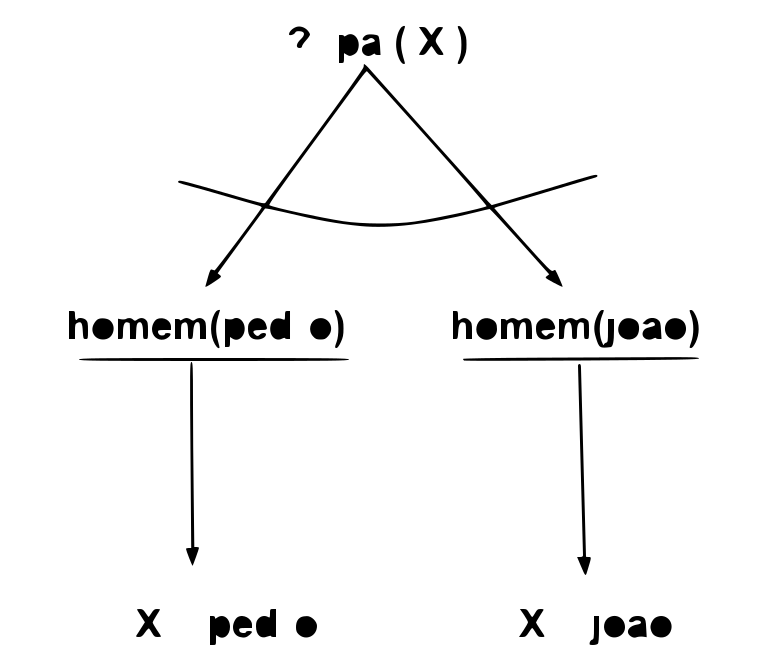
\includegraphics[scale = 0.2]{figuras/fluxo-da-maquina-prolog-01.pdf}
\label{fig_fluxo_px}
\caption{Fluxo básico de um predicado em Prolog.}
\end{figure}

\end{block}   
\end{frame}

%%%%%%%%%%%%%%%%%%%%%%%%%%%%%%%%%%%%%%%%%%%%%%%%%
\begin{frame}[fragile]
\begin{block}{Exemplo de Regra}


%\inputminted[firstline=2, lastline=12]{Prolog}{prolog/exemplo-01.pl}
\begin{comment}
%\begin{lstlisting}
\lstinputlisting[language=Prolog, 
                  basicstyle=\footnotesize\ttfamily,
                  backgroundcolor=\color{azulclaro}, 
                  keywordstyle=\color{red},   
                  keepspaces=true, 
                  lineskip = -2pt, % espacamento entre linhas
%%                  numbersep=5pt   
                  keywordstyle=\color{magenta},
     numberstyle=\tiny\color{magenta},
     commentstyle=\color{green},             
    numbers=left, 
    captionpos = b, % posiaodo caption 
    label={code-dados-pessoais}, 
    caption={Exemplo de Regra}                 
    ]{prolog/exemplo-01.pl}
%\end{lstlisting}
\end{comment}

{\scriptsize
\inputminted{Prolog}{prolog/exemplo-01.pl}
}

\end{block}

\end{frame}




\begin{frame}
\begin{block}{Funcionamento de uma Regra}

\begin{figure}[!htb]
\centering
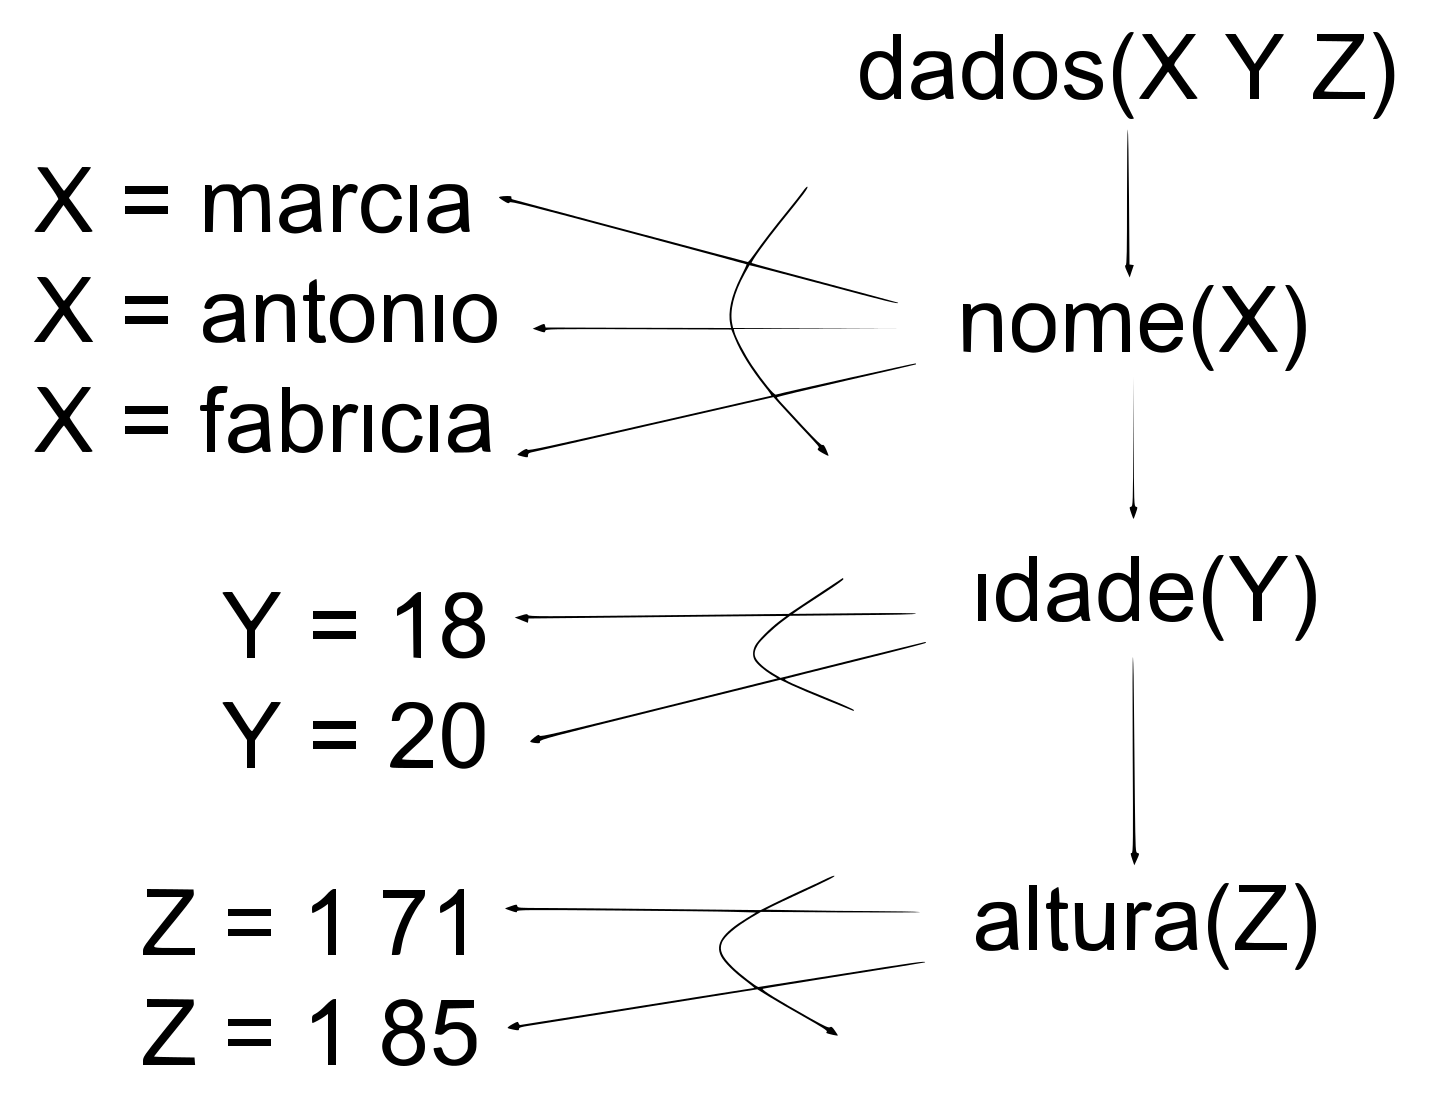
\includegraphics[width=0.5\textwidth , height=0.5\textheight]{figuras/fluxocomposto.pdf}
\label{fig_fluxocomposto}
\caption{Fluxo básico de uma regra em Prolog}
\end{figure}

\end{block}   
\end{frame}

\begin{frame}
\frametitle{Execução:}
\begin{figure}[!htb]
\centering
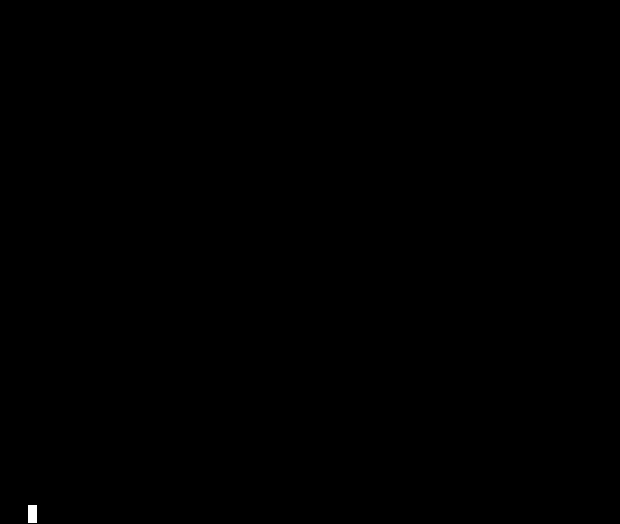
\includegraphics[width=0.85\textwidth , height=0.7\textheight]{figuras/prologcomposto.pdf}
\label{fig_fluxo_pxyz_execucao}
\end{figure}
\end{frame}

%%%%%%%%%%%%%%%%%%%%%%%%%%%%%%%%%%%%%%%%%%%%%%%%%

%\section{Resumo da 1a. Parte} 
%%%% Uma seção pode ser composta de varios frames...
\begin{frame}[fragile]   %%%% indica que o ambiente  FRAME é frágil

\begin{block}{Resumo até o momento:}

\begin{itemize}
\item Precisamos de um editor de programas e um compilador
\item $3$ elementos compõem a sintaxe do Prolog: \textbf{fatos}, \textbf{regras} e \textbf{questões}
\item \textbf{Fatos}: expressam dados conhecidos ou verdades incondicionais
\item \textbf{Regras}: expressam conhecimentos genéricos, como regras gerais dos fatos.
\item Um conhecimento é uma uma verdade condicional, isto é, uma regra ou
fato que precisa ser provado
\item \textbf{Questões}: buscam fazer a demonstrações das verdades de regras e fatos
\item Pratique!
\item Voce já pode criar e resolver muitos problemas difíceis e interessantes
\item Exemplos: \url{https://github.com/claudiosa/prolog}
\end{itemize}

\end{block}
\end{frame}

\begin{frame}[fragile]   %%%% indica que o ambiente  FRAME é frágil
\frametitle{Pausa}

\begin{figure}[!htb]
\centering
\includegraphics[width=0.85\textwidth , height=0.65\textheight]{figuras/the_end_video.png}
%%Prolog/
%\label{fig_functor_termo}
%\caption{Um exemplo de functor -- um termo composto.}
\end{figure}



\end{frame}

%%%%%%%%%%%%%%%%%%%%%%%%%%%%%%%%%%%%%%%%%%%%%%%%%%%%%%%%%%%%


\section{Functores ou Funções Lógicas} 
%%%% Uma seção pode ser composta de varios frames...
\begin{frame}[fragile]   %%%% indica que o ambiente  FRAME é frágil
\frametitle{Functores ou Funções Lógicas}


\begin{block}{Nesta vídeo-aula}
\begin{itemize}
\itemsep 0.5cm

\item Conceito sobre Functores
\item Dois exemplos
\item Pré-requisito: \textbf{fatos}, \textbf{questões} e \textbf{regras}
\item Ao final: \textit{prontos} para resolverem os problemas do sítio \url{http://rachacuca.com.br/}
\item Todos os códigos aqui discutidos estão: \url{https://github.com/claudiosa/prolog}
\item A apresentação: \url{http://www2.joinville.udesc.br/~coca/index.php/Main/LogicaMatematica}
\end{itemize}

\end{block}   
\end{frame}


%\textcolor{red}{Muito boa sequência aqui ....}
%%%%%%%%%%%%%%%%%%%%%%%%%%%%%%%%%%%%%%%%%%%%%%%%%%%%%%%%%%%%%%%
\begin{frame}[fragile]   %%%% indica que o ambiente  FRAME é frágil
\frametitle{Functores}

\begin{block}{Conceito:}
\begin{itemize}
\itemsep 0.4cm

\item Functores são termos compostos  utilizados para representar funções 
com termos combinados entre si.

\item Assim, o functor é um termo da relação e internamente  há outros termos e átomos.  

\item Uma estratégia de contornar o \textbf{V}erdadeiro  ou \textbf{F}also da LPO e/ou do Prolog
\item Exemplos:
\end{itemize}

\begin{enumerate}
%\itemsep 0.5cm

% \item \texttt{+(1,2): 1+2}
% \item \texttt{magro(paulo): Paulo é magro}
\item \texttt{pai(pedro, joao)}: Pedro é o pai do João
\item mas \texttt{pai(pai(pedro), filho(joao))}: é muito diferente
\item Pois: $pai(pedro) \mapsto adao$  e  $filho(joao) \mapsto abel$
\end{enumerate}

\end{block}   
\end{frame}

\begin{frame}
\begin{block}

\begin{figure}[!htb]
\centering
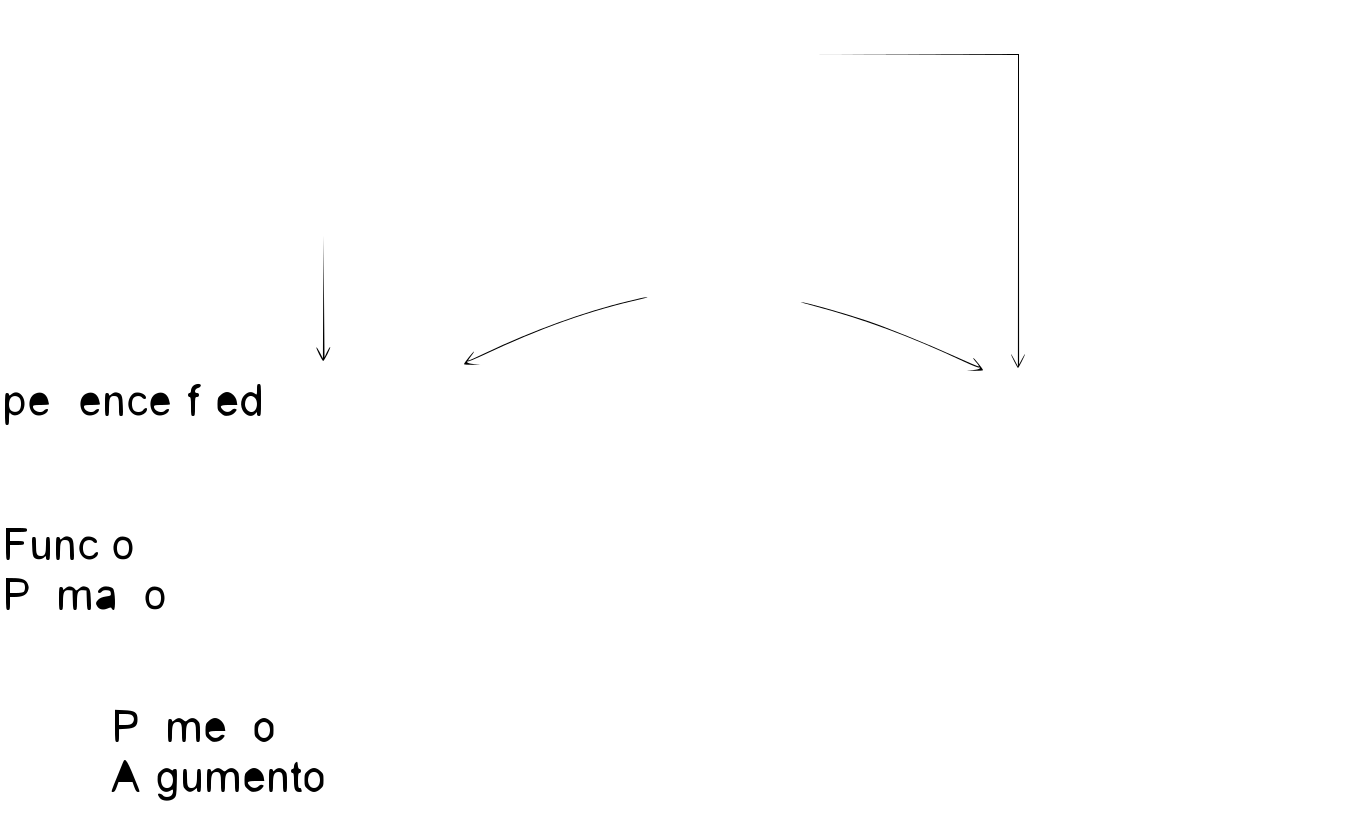
\includegraphics[scale = 0.22]{figuras/functorcomposto.pdf}
%%Prolog/
\label{fig_functor_termo}
\caption{Um exemplo de functor -- um termo composto.}
\end{figure}

\end{block}   
\end{frame}

\begin{frame}[fragile]
\begin{block}{Código:}

\begin{lstlisting}[language=Prolog, 
                   basicstyle=\footnotesize\ttfamily,
                  backgroundcolor=\color{azulclaro}, 
                  keywordstyle=\color{red},   
                  keepspaces=true,    
                  keywordstyle=\color{magenta},
     numberstyle=\tiny\color{magenta},
     commentstyle=\color{green},             
    numbers=left,                    
    numbersep=5pt]
carros :- 
  pertence(X,Y,Z)

pertence(fred, 
  carro(fabricante(toyota, japao)), 
  ano_cor(2014, azul)).
  
pertence(romi, 
  carro(fabricante(bmw, alemanha)), 
  ano_cor(2015, vermelho)).
  
pertence(claudio, 
  carro(fabricante(vw, brasil)), 
  ano_cor(2012, prata)).
\end{lstlisting}
\end{block}
\end{frame}

\begin{frame}
\frametitle{Execução:}

\begin{figure}[!htb]
\centering
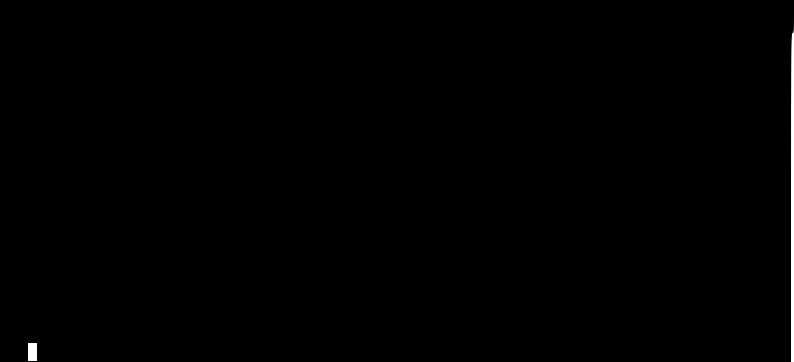
\includegraphics[width=0.85\textwidth , height=0.65\textheight]{figuras/carros1.pdf}
\label{fig_carros1}
\end{figure}
   
\end{frame}

\begin{frame}
\frametitle{Execução com Condicional:}

\begin{figure}[!htb]
\centering
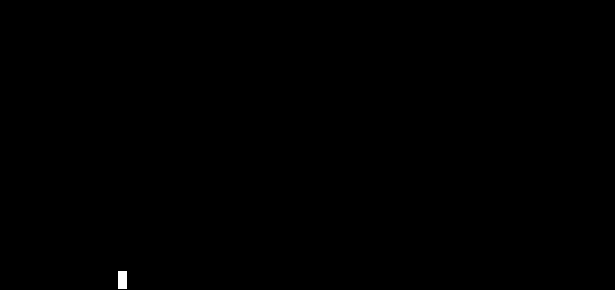
\includegraphics[width=0.85\textwidth , height=0.5\textheight]{figuras/carros2.pdf}
\label{fig_carros2}
\caption{A pergunta foi feita com \textbf{uma condição}: \texttt{A > 2014}}
\end{figure}
 
\end{frame}


\begin{frame}[fragile]   %%%% indica que o ambiente  FRAME é frágil
\frametitle{Pausa}

\begin{figure}[!htb]
\centering
\includegraphics[width=0.85\textwidth , height=0.65\textheight]{figuras/the_end_video.png}
%%Prolog/
%\label{fig_functor_termo}
%\caption{Um exemplo de functor -- um termo composto.}
\end{figure}

\end{frame}
%%%%%%%%%%%%%%%%%%%%%%%%%%%%%%%%%%%%%%%%%%%%%%%%%%%%%%%%

\begin{frame}[fragile]   %%%% indica que o ambiente  FRAME é frágil
\frametitle{Exercícios}
\begin{block}{Identifique o que os fatos representam:}

\begin{enumerate}

\item \texttt{animal(gato)}
\item \texttt{veiculo(moto)}
\item \texttt{cor(preta)}
\item \texttt{mãe(maria,bia)}
\item \texttt{móvel(Sofá)}

\end{enumerate}
\end{block}   
\end{frame}

\begin{frame}[fragile]   %%%% indica que o ambiente  FRAME é frágil
\frametitle{Exercícios}
\begin{block}{Identifique o que os fatos representam:}

\begin{enumerate}

\item \texttt{animal(gato)} - {\bf gato é um animal}
\item \texttt{veiculo(moto)} - {\bf moto é um veiculo}
\item \texttt{cor(preta)} - {\bf preto é uma cor}
\item \texttt{mãe(maria,bia)} - {\bf maria é mãe da bia}
\item \texttt{móvel(Sofá)} -  \textcolor{red}{CUIDADO} {\bf não significa que sofá é um movel porque Sofá é uma variável}


\end{enumerate}
\end{block}   
\end{frame}

%%%%%%%%%%%%%%%%%%%%%%%%%%%%%%%%%%%%%%%%%%%%%%%%%

\section{Recursividade} 
%%%% Uma seção pode ser composta de varios frames...
\begin{frame}[fragile]   %%%% indica que o ambiente  FRAME é frágil
\frametitle{Recursividade}

 
\begin{figure}[!htb]
\centering
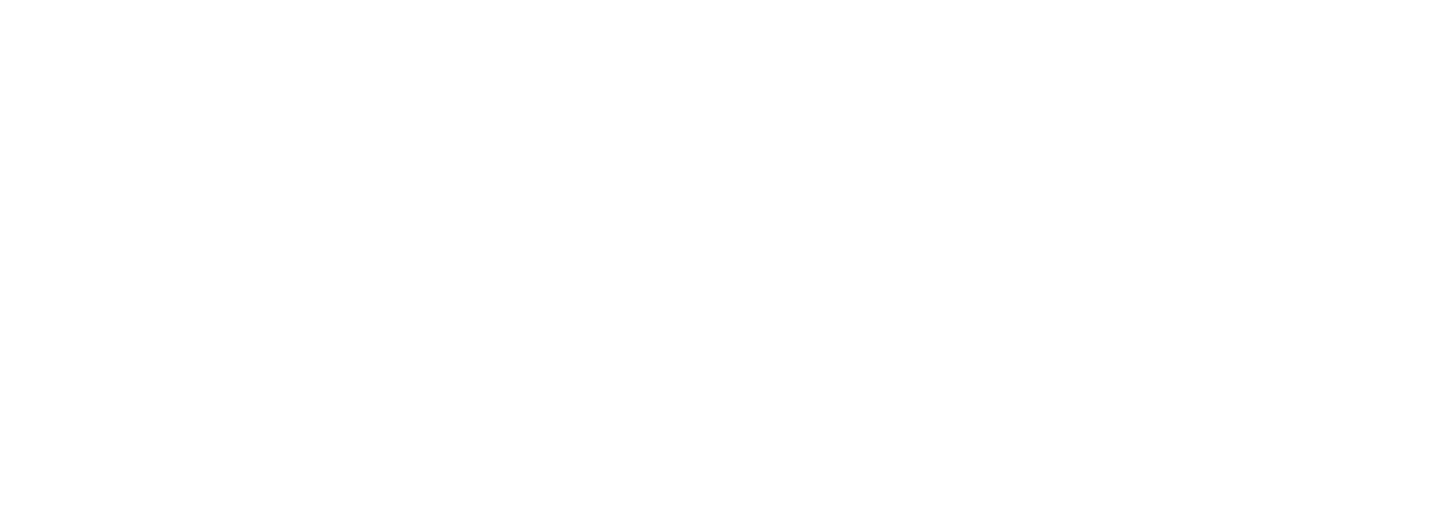
\includegraphics[scale = 0.2]{figuras/recursividade_ilustra_1.pdf}
%\includesvg[svgpath = figuras/, width = 0.5\textwidth, height = 0.6%%\textheight]{recursividade_ilustra_1}
%%Prolog/
\label{fig_recursividade_ilustra_1}
\caption{Recursão ilustrada}
\end{figure}
 
   
\end{frame}







%%%%%%%%%%%%%%%%%%%%%

\begin{frame}
\begin{block}{Conceito:}
\begin{itemize}

\item A recursão é um conceito importante da linguagem Prolog.

\item Esta permite expressar problemas complexos de uma maneira simples.

\item Um exemplo  é a relação \texttt{descendente(X,Y)} ``\textit{Y é um descendente de X}''. 

\item Esta definição utiliza a relação \texttt{genitor} que é uma
descendência direta, ou seja, quando \texttt{X} é genitor de \texttt{Y}, 
é representada com a seguinte regra:\\

\texttt{descendente(X,Z) :- genitor(X,Z)}.

\end{itemize}
\end{block}   
\end{frame}
%%%%%%%%%%%%%%%%%%%%%%%%%%%%%%%%%%%%%%%%%%%%%%%%%%%%%

\begin{frame}

\begin{block}{Outros Casos:}
\begin{itemize}
\itemsep 17pt

\item Outros casos de descendência, que não uma descendência direta, poderiam ser
utilizadas seguintes regras:

%%\item \textcolor{red}{Escrever diretamente o que é o PONTO  ....}

\begin{enumerate}
\item \texttt{descendente(X,Z) :- genitor(X,Y) , genitor(Y,Z).}

\item \texttt{descendente(X,Z) :- ancestral(Z,X).}

\item Claro: o conceito de \texttt{ancestral} é o oposto de \texttt{descendente}
\end{enumerate}
%%%% \item Entretanto, essa forma é trabalhosa. 

\item Usando recursão é possível obter uma
solução simples. Para isso, é
necessário definir a seguinte afirmação: \texttt{X} é um descendente de Z se existe um Y, tal que,
X seja genitor de Y e Y seja um descendente de Z, a seguinte regra descreve isso:\\
\texttt{descendente(X,Z) :- genitor(X,Y) , descendente(Y,Z).}

%\item \textcolor{red}{Rever esta parte após o código pronto}
%\item \textcolor{red}{veja meu codigo de ancestral}


\end{itemize}
\end{block}   
\end{frame}

%%%%%%%%%%%%%%%%%%%%%%%%%%%%%%%%%%%%%%%

\begin{frame}[fragile]
\begin{block}{Problema: Árvore Genealógica}
%\textcolor{red}{Mover para cima}
\begin{figure}[!htb]

\centering
\includegraphics[scale = 0.17]{figuras/ArvoreProlog.pdf}
%%Prolog/
\label{fig_functor_termo}
\caption{Árvore Genealógica}

\end{figure}
\end{block}
\end{frame}
 %%%%%%%%%%%%%%%%%%%%%%%%%%%%%%%%%%%%%%%%%%%%%%%%%%%%%%%%

\begin{frame}[fragile]
\begin{block}{Programa:}
\begin{itemize}
 \item O programa completo que descreve as relações familiares discutidas nesta seção pode
ser observado a seguir:
\end{itemize}

\begin{lstlisting}[language=Prolog, 
                   basicstyle=\footnotesize\ttfamily,
                  backgroundcolor=\color{azulclaro}, 
                  keywordstyle=\color{red},   
                  keepspaces=true,    
                  keywordstyle=\color{magenta},
     numberstyle=\tiny\color{magenta},
     commentstyle=\color{green},             
    numbers=left,                    
    numbersep=5pt]
ancestral(ana,maria).
ancestral(pedro,maria).
ancestral(maria,paula).
ancestral(paula,lucas).
mulher(ana).
mulher(maria).
mulher(paula).
homem(pedro).
homem(lucas).
prole(Y,X) :- ancestral(X,Y).
mae(X,Y) :- ancestral(X,Y), mulher(X). 
avos(X,Z) :- ancestral(X,Y), ancestral(Y,Z). 
descendente(X,Z) :- ancestral(X,Z).
descendente(X,Z) :- ancestral(X,Y), descendente(Y,Z).
\end{lstlisting}    

\end{block}
\end{frame}

%%%%%%%%%%%%%%%%%%%%%%%%%%%%%%%%%%%%%%%

\begin{frame}
\frametitle{Testando Programa:}

\begin{figure}[!htb]
\centering
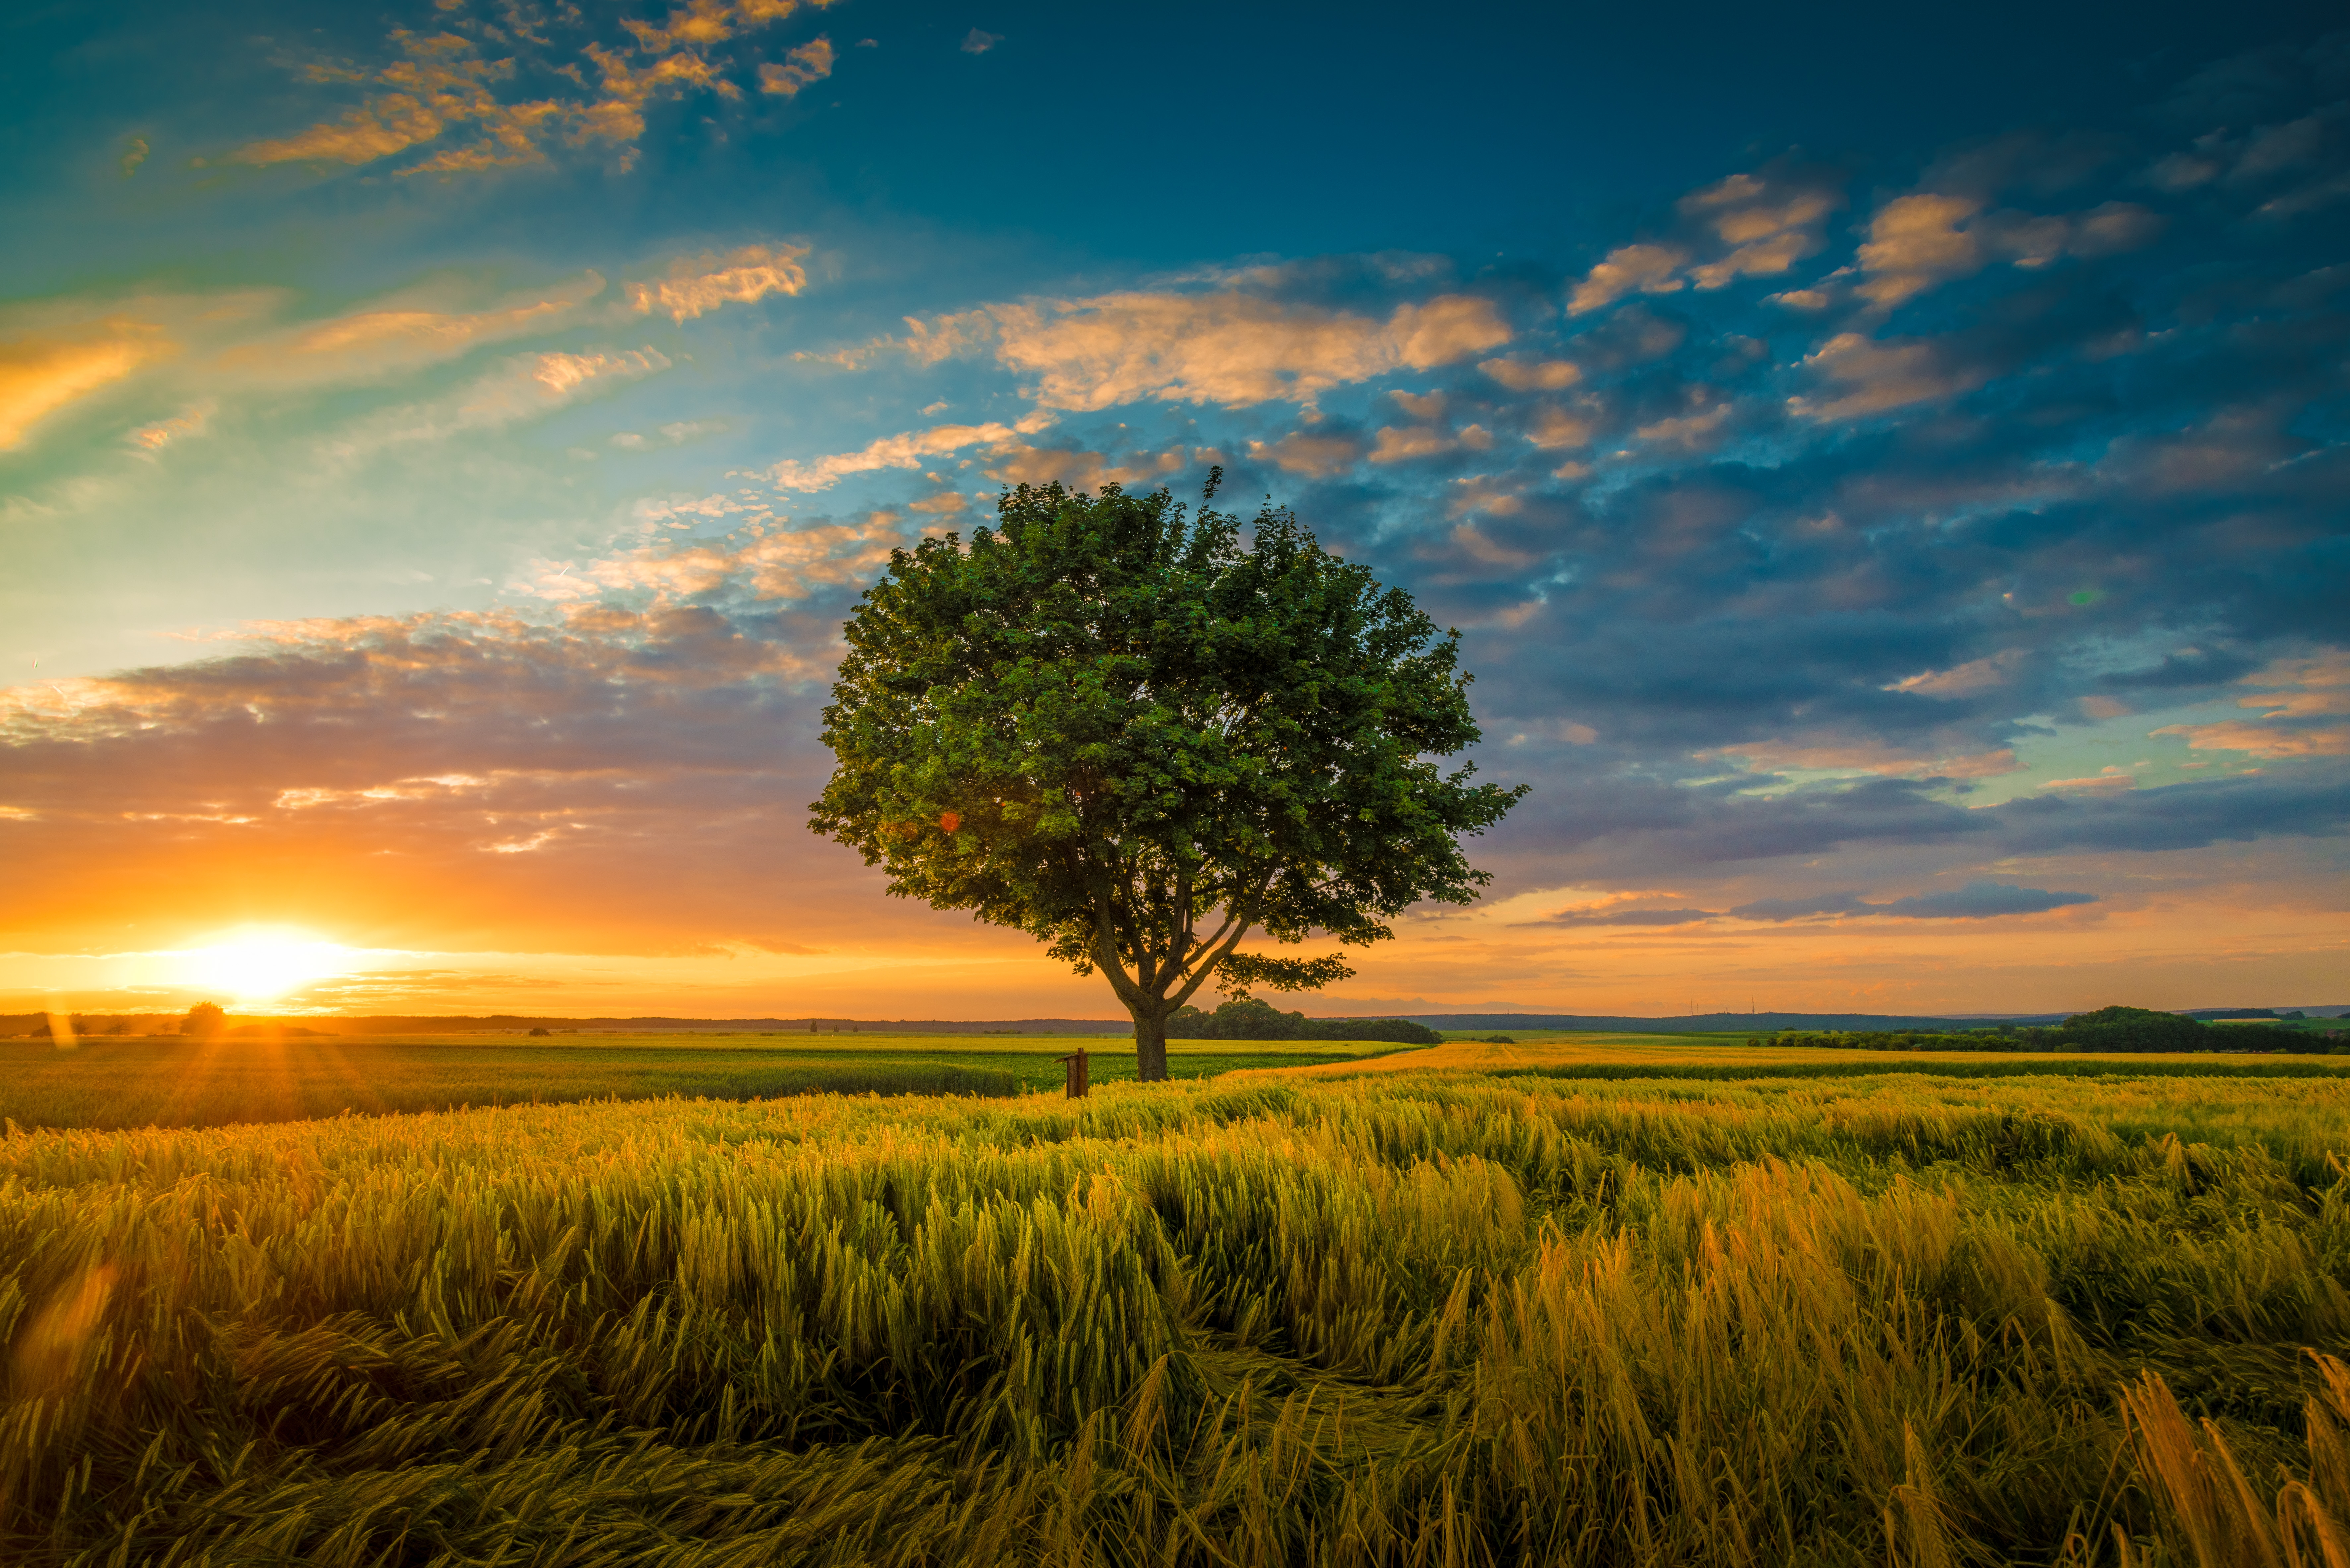
\includegraphics[width=0.85\textwidth , height=0.65\textheight]{figuras/arvore.pdf}
%%Prolog/
\label{fig_recurs_3}
%\caption{\url{http://swish.swi-prolog.org}}
\end{figure}

\end{frame}

\begin{frame}[fragile]
\begin{block}{Resultado:}
\begin{itemize} 
\item A consulta a seguir um exemplo sobre a relação de descendência, nela exibe todos os descendentes de Ana:
\end{itemize}

\begin{lstlisting}[language=Prolog, 
                   basicstyle=\footnotesize\ttfamily,
                  backgroundcolor=\color{azulclaro}, 
                  keywordstyle=\color{red},   
                  keepspaces=true,    
                  keywordstyle=\color{magenta},
     numberstyle=\tiny\color{magenta},
     commentstyle=\color{green},             
    numbers=left,                    
    numbersep=5pt]
?- descendente (ana,X).
X = maria;
X = paula;
X = lucas;
false.
\end{lstlisting}
\end{block}
\end{frame}

%%%%%%%%%%%%%%%%%%%%%%%%%%%%%%%%%%%%%%%%%%%%%

\begin{frame}[fragile]
\begin{block}{Soma Recursiva}

\[
S(n)=1+2+3+4+.....+(n-1)+n
\]

Este problema é reformulado sob uma visão matemática, mais
especificamente, pela \textit{indução finita} dada por:


\[
S(n)=\left \{
\begin{tabular}
[c]{ll}
$1$ & para $n=1$ \\
$S(n-1) + n $ & para $n \geqslant 2$
\end{tabular}
\right.
\]


\end{block}
\end{frame}


\begin{frame}[fragile]
\begin{block}{Soma Recursiva}

O que \'{e} um fato verdadeiro pois:

\[
S(n)=
\begin{tabular}[c]{cc}
$\underbrace{1+2+3+.....+(n-1)}$ &  $  + n$\\
$S(n-1)$ &
\end{tabular}
\]

Como o procedimento é recursivo, é necessário encontrar a definição da ``\textbf{parada}'' da recursividade. 

Como $n$ não tem limite superior, é para qualquer $n$, inicia-se pelo que se conhece:
{\small
\begin{center}
\begin{tabular}[l]{p{0.7\textwidth}}\hline\hline
\textbf{\#1}. A soma de 1 \'{e} 1, logo: soma(1,1).\\
\textbf{\#2}. Para soma dos $n$-\'{e}simos termos, \'{e} necess\'{a}rio
 a soma do $(n-1)$-\'{e}simos termos, logo:\\
soma(N,S) ... = ... Nant = (N-1), soma(Nant, S\_Nant)\\
 e S = (N + S\_Nant).\\\hline\hline
\end{tabular}
\end{center}
}


\end{block}
\end{frame}


\begin{frame}[fragile]
\begin{block}{Soma  Recursiva}

{\small
\inputminted{Prolog}{prolog/soma2.pl}
}

\begin{comment}
\lstinputlisting[language=myPrologstyle, 
                  basicstyle=\footnotesize\ttfamily,
                  backgroundcolor=\color{azulclaro}, 
                  keywordstyle=\color{red},   
                  keepspaces=true, 
                  lineskip = -2pt, % espacamento entre linhas
                  numbersep=5pt   
                  keywordstyle=\color{magenta},
     numberstyle=\tiny\color{magenta},
     commentstyle=\color{green},             
    numbers=left, 
    captionpos = b, % posiaodo caption 
    label={soma}, 
    caption={Soma}                 
    ]{prolog/soma2.pl}
\end{comment}    
\end{block}

\end{frame}

%%%%%%%%%%%%%%%%%%%%%%%
\begin{frame}
\frametitle{Execução s(7,7):}

\begin{figure}[!htb]
\centering
\includegraphics[scale = 0.65]{figuras/soma1.pdf}
\label{soma1}
\end{figure}

  
\end{frame}

%%%%%%%%%%%%%%%%%%%%%%%%%%%%%%%%%%%%%%%%%%%%%%%%%%%%%%

\begin{frame}
\frametitle{Execução s(5,x):}

\begin{figure}[!htb]
\centering
\includegraphics[width=0.85\textwidth , height=0.65\textheight]{figuras/soma2.pdf}
\label{soma2}
\end{figure}
 
\end{frame}

\begin{frame}[fragile]   %%%% indica que o ambiente  FRAME é frágil
\begin{block}{Exercício:}
\begin{itemize}

\item Crie fatos e uma regra e faça uma consulta no swi-prolog para ver o resultado.

\end{itemize}
\end{block}   
\end{frame}

%%%%%%%%%%%%%%%%%%%%%%%%%%%%%%%%%%%%%%%%%%%%%%%%%

\begin{frame}
\frametitle{Fatorial}
\begin{block}{Definição:}
\begin{itemize}
\item Reformulando sob uma visão
matemática, mais especificamente, pela indução finita tem-se:
\[
Fat(n)=\left\{
\begin{tabular}[c]{ll}%
$1$ & para $n=0$\\
$Fat(n-1)\ast n$ & para $n\geqslant1$%
\end{tabular}
\right.
\]
\vskip 11pt
O que \'{e} um fato verdadeiro pois:
\vskip 11pt
\[
Fat(n)=
\begin{tabular}
[c]{cc}%
$\underbrace{1\ast2\ast3\ast.....\ast(n-1)}$ & $\ast \ n$\\
$Fat(n-1)$ &
\end{tabular}
\]

Como o procedimento é recursivo, deve-se encontrar a definição para
``\textbf{parada}'' da recursividade. Como $n$ não tem limite superior, é para qualquer $n$, então inicia-se pelo que se conhece:

\end{itemize}
\end{block}
\end{frame}

%%%%%%%%%%%%%%%%%%%%%%%%%%%%%%%%%%%%%%%%%%%%%%%%%

\begin{frame}
\begin{block}{}
\begin{center}%
\begin{tabular}
[c]{|l|}\hline
\textbf{\#1}. O fatorial de 0 \'{e} 1, logo: fatorial(0,1).\\
\textbf{\#2}. O fatorial  do $n$-\'{e}simo termo, \'{e} necess\'{a}rio \\
o fatorial do $(n-1)$-\'{e}simo termo, logo:\\
fatorial(N, Fat) ::  Nant = (N-1), fatorial(Nant, Fat\_Nant) e \\
 Fat = (N $\ast$ Fat\_Nant).\\ \hline
\end{tabular}
\end{center}
\end{block}
\end{frame}
%%%%%%%%%%%%%%%%%%%%%%%%%%%%%%%%%%%%%%%%%%%%%%%%%

\begin{frame}
\begin{block}{Em termos de Prolog tem-se:}

\lstinputlisting[language=Prolog, 
                  basicstyle=\footnotesize\ttfamily,
                  backgroundcolor=\color{azulclaro}, 
                  keywordstyle=\color{red},   
                  keepspaces=true, 
                  lineskip = -2pt, % espacamento entre linhas
%%                  numbersep=5pt   
                  keywordstyle=\color{magenta},
     numberstyle=\tiny\color{magenta},
     commentstyle=\color{green},             
    numbers=left, 
    captionpos = b, % posiaodo caption 
    label={fatorial},                 
    ]{prolog/fatorial2.pl}

\end{block}
\end{frame}

\begin{frame}[fragile]
\frametitle{Exercício:}
\begin{block}{Complete a tabela abaixo, para descrição do fatorial:}

{\small
\begin{center}
\begin{tabular}
[c]{|l|l|l|l|l|l|}\hline
\textbf{Chamada Pendente} & \textbf{Regra Casada} & \textbf{X} & \textbf{Aux} & \textbf{Parcial} & \textbf{Fat} \\ \hline
{\small fatorial}(5,X) & \# & ...... & ...... & ?...... $\rightarrow$ &
......\\\hline
{\small fatorial}(4,X) & \# & ...... & ...... & ?...... $\rightarrow$ &
$\nwarrow$......\\\hline
{\small fatorial}(3,X) & \# & ...... & ...... & ?...... $\rightarrow$ &
$\nwarrow$......\\\hline
{\small fatorial}(2,X) & \# & ...... & ...... & ?...... $\rightarrow$ &
$\nwarrow$......\\\hline
{\small fatorial}(1,X) & \# & ...... & ...... & ?...... $\rightarrow$ &
$\nwarrow$......\\\hline
{\small fatorial}(0,X) & \# & ...... & ...... & ?...... $\rightarrow$ &
$\nwarrow$......\\\hline
\end{tabular}
\end{center}
}

\end{block}   
\end{frame}

%%%%%%%%%%%%%%%%%%%%%%%%%%%%%%%%%%%%%%%%%%%%%%%%%

\begin{frame}[fragile]   %%%% indica que o ambiente  FRAME é frágil

\frametitle{FALTA AINDA}

\begin{enumerate}
 \item \textcolor{red}{Paulo: corrigi até aqui .... }

  \item \textcolor{red}{ Há outros exemplos de recursividade na apostila original, prontos, como o fatorial ou do ancestral... que está muito legal. Siga o modelo aplicado.}

  \item \textcolor{red}{TODAS figuras devem ser em formato VETORIAL: pdf ou svg}
  
  \item \textcolor{red}{png ... não é vetorial.... salve em pdf ou svg ou use um conversor como: \url{http://vectormagic.com/support/file_formats}}

 \textcolor{red}{Cuidar mais com a Língua Portuguesa .. há muitos erros no texto de acentuação Básica}

\item \textcolor{red}{A figura da próxima página é inadmissível}


\item \textcolor{red}{Não apague estas observações}

\end{enumerate}
\end{frame}



%%%%%%%%%%%%%%%%%%%%%%%%%%%%%%%%%%%%%%%%%%%%%%%%%
\section{Listas}

\begin{frame}[fragile]   %%%% indica que o ambiente  FRAME é frágil
\frametitle{Listas}


\begin{block}
 
\begin{figure}[!htb]
\centering
\includegraphics[scale = 0.6]{figuras/ListaDados.png}
\end{figure}
 
\end{block}   
\end{frame}

%%%%%%%%%%%%%%%%%%%%%%%%%%%%%%%%%%%%%%%%%%%%%%%%%
%%%% Uma seção pode ser composta de varios frames...
\begin{frame}[fragile]   %%%% indica que o ambiente  FRAME é frágil
\frametitle{Listas}

%\textcolor{red}{Uma figura mais ilustrativa}

%\begin{block}
 
\begin{figure}[!htb]
\centering
\includegraphics[scale = 0.3]{figuras/lista2.pdf}
\caption{[1, 3, 7, 11]}
\end{figure}
 
%\end{block}   
\end{frame}

%%%%%%%%%%%%%%%%%%%%%%%%%%%%%%%%%%%%%%%%%%%%%%%%%%%%%

\begin{frame}
\begin{block}{Listas}
\begin{itemize}

\item Pré-requisito: conceitos de recursividade e functor dominados!
\item Seguem conceitos das LPs convencionais
\item Essencialmente vamos computar sob uma árvore binária
\item Ilustrando esta computação 

\end{itemize}
\end{block}   
\end{frame}

%%%%%%%%%%%%%%%%%%%%%%%%%%%%%%%%%%%%%%%%%%%%%%%%%%%%%%%

\begin{frame}
\frametitle{Fluxo Operacional das Listas}

\begin{figure}[!htb]
\centering
\includegraphics[scale = 0.25]{figuras/FluxoOperacional.png}
%%Prolog/
\label{fig_arv_recurs_2}
\caption{Cálculo Recursivo 2}
\end{figure}

  %\textcolor{red}{Esta figura DEVE ser modificada} 

\end{frame}

%%%%%%%%%%%%%%%%%%%%%%%%%%%%%%%%%%%%%%%%%%%%%%%%%%%%

\begin{frame}
\frametitle{Definições}
\begin{block}{Uma lista é:}
\begin{itemize}

\item Uma estrutura de dados que representa uma coleção de objetos homogêneos;
\item Uma sequência de objetos;
\item Um  tipo particular de functor
\footnote{{\bf Logo, a lista apresenta uma hierarquia natural, 
internamente recursiva.}} (veja esta nota de roda-pé), 
pois apresenta uma hierarquia interna.
\item {\bf Notação:} O símbolo ``\lbrack'' é usado para descrever o início de uma lista,
e ``\rbrack'' para o final da mesma;

\end{itemize}
\end{block}   
\end{frame}

%%%%%%%%%%%%%%%%%%%%%%%%%%%%%%%%%%%%%%%%%%%%%%%%

\begin{frame}
\begin{block}{Exemplos:}

\begin{itemize}
  \item \lbrack a, b, c, d \rbrack,  logo um predicado cujo
argumento seja algumas letras,  tem-se uma lista do tipo:
\end{itemize}

\lstinputlisting[language=Prolog, 
                  basicstyle=\footnotesize\ttfamily,
                  backgroundcolor=\color{azulclaro}, 
                  keywordstyle=\color{red},   
                  keepspaces=true, 
                  lineskip = -2pt, % espacamento entre linhas
%%                  numbersep=5pt   
                  keywordstyle=\color{magenta},
     numberstyle=\tiny\color{magenta},
     commentstyle=\color{green},             
    numbers=left, 
    captionpos = b, % posiaodo caption 
    label={cabecalista},                 
    ]{prolog/cabecalista.txt}

\begin{itemize}
\item Os elementos de uma lista são lidos da esquerda para direita, logo a letra
``a'' é o primeiro elemento ou ``{\em cabeça}'' da lista. Quanto ao
resto ou ``{\em cauda}'' da lista, é uma   ``{\em sub-lista}''  dada por:
\lbrack b,  c, d \rbrack.  Esta sub-lista também é uma lista.
\end{itemize}
\end{block}   
\end{frame}

\begin{frame}
\begin{block}{Exemplos:}


{\bf Operador Pipe:} define quem é a cabeça da cauda da lista. 
Ele é simbolizado por ``{\bf |}'', que distingue a parte da esquerda da direita da lista. 
Isto é necessário para se realizar os casamentos de padrões com as variáveis.

\end{block}   
\end{frame}

%%%%%%%%%%%%%%%%%%%%%%%%%%%%%%%%%%%%%%%

\begin{frame}
\begin{block}{Exemplos:}

{\bf Exemplos de ``casamentos'':} os exemplos abaixo definem
como ocorrem os casamentos entre variáveis e listas.
Faça suas próprias conclusões de como as listas operam.

\end{block}

\lstinputlisting[language=Prolog, 
                  basicstyle=\footnotesize\ttfamily,
                  backgroundcolor=\color{azulclaro}, 
                  keywordstyle=\color{red},   
                  keepspaces=true, 
                  lineskip = -1pt, % espacamento entre linhas
                  numbers=left, 
                  numbersep=-7pt,   
                  keywordstyle=\color{magenta},
                  tabsize=2,	                   % sets default tabsize to 2 spaces
     numberstyle=\tiny\color{magenta},
     commentstyle=\color{green},             
    captionpos = b, % posiaodo caption 
    label={casamento},                 
    ]{prolog/casamento.txt}


\end{frame}

%%%%%%%%%%%%%%%%%%%%%%%%%%%%%%%%%%%%%%%
\begin{frame}
\begin{block}{Auto-Definição}
\begin{itemize}

\item Retomando ao conceito de listas,
se ``{\em auto-define}''  o conceito de lista com os seguintes axiomas:

\begin{enumerate}
%\setlength{\itemsep}{-5pt}
\item   {\em Uma lista vazia é uma lista};
\item   {\em  Uma sub-lista é uma lista}.
\end{enumerate}

\item As definições acima são recorrentes, isto é, uma depende da outra. Em outras  palavras, Reescrenvendo em Prolog tal definição é dada por:

\lstinputlisting[language=Prolog, 
                  basicstyle=\footnotesize\ttfamily,
                  backgroundcolor=\color{azulclaro}, 
                  keywordstyle=\color{red},   
                  keepspaces=true, 
                  lineskip = -2pt, % espacamento entre linhas
%%                  numbersep=5pt   
                  keywordstyle=\color{magenta},
     numberstyle=\tiny\color{magenta},
     commentstyle=\color{green},             
    numbers=left, 
    captionpos = b, % posiaodo caption 
    label={lista},                 
    ]{prolog/lista.txt}

\end{itemize}
\end{block}
\end{frame}

%%%%%%%%%%%%%%%%%%%%%%%%%%%%%%%%%%%%%%%

\begin{frame}
%\frametitle{Mapa de Memória}

\begin{block} {Mapa de Memória}

\begin{center}{
\begin{tabular}
[c]{c|c|c|c}\hline \hline
& \textbf{Regra} & \textbf{X} & \textbf{T}\\ \hline \hline
eh\_uma\_lista([a,b,c]) & \#2 & a & [b,c]\\ \hline
eh\_uma\_lista([b,c]) & \#2 & b & [c]\\ \hline
eh\_uma\_lista([c]) & \#2 & c & []\\ \hline
eh\_uma\_lista([]) & \#1 & -- & --\\ \hline \hline
\end{tabular}}
\end{center}

  Basicamente, quase todas operações com listas possuem regras análogas a definição acima. 
 O exemplo anterior serve apenas para identificar que o  objeto: \lbrack a,b,c,d \rbrack ,  é uma lista.

\end{block}   
\end{frame}

%%%%%%%%%%%%%%%%%%%%%%%%%%%%%%%%%%%%%%%%%%%%%%%%%%%%

\begin{frame}
\begin{block}{Exemplos de lista}

  As regras sobre listas são diversas e elegantes. Apenas exercitando
há que se cria a destreza para resolve-las.
Alguns  clássicos são mostrados nos exemplos que se seguem. Há alguns
que são combinados com outros criando alguns bem complexos.

\end{block}
\end{frame}

%%%%%%%%%%%%%%%%%%%%%%%%%%%%%%%%%%%%%%%%%%%%%%%%%%%%

\begin{frame}
\begin{block}{Comprimento de uma lista:}

  O comprimento de uma lista é o comprimento de sua sub-lista, mais um,
sendo que o comprimento de uma lista vazia é zero. Em Prolog
isto é dado por:


\lstinputlisting[language=Prolog, 
                  basicstyle=\footnotesize\ttfamily,
                  backgroundcolor=\color{azulclaro}, 
                  keywordstyle=\color{red},   
                  keepspaces=true, 
                  lineskip = -2pt, % espacamento entre linhas
%%                  numbersep=5pt   
                  keywordstyle=\color{magenta},
     numberstyle=\tiny\color{magenta},
     commentstyle=\color{green},             
    numbers=left, 
    captionpos = b, % posiaodo caption 
    label={lista},                 
    ]{prolog/lista2.txt}

\end{block}
%\textcolor{red}{Um por frame, tirar \#, e a execução .... em figura... }
\end{frame}

%%%%%%%%%%%%%%%%%%%%%%%%%%%%%%%%%%%%%%%

\begin{frame}
%\frametitle{Mapa de Memória}

\begin{block} {Mapa de Memória}

\begin{center}{
\begin{tabular}[c]{c|c|c|c|c|c}
\hline \hline
& \textbf{Regra} & \textbf{X} & \textbf{T} & \textbf{N1} & \textbf{N is N+1}\\ \hline \hline
compto([a,b,c,d],N) & \#2 & a & [b,c,d] & 3 $\rightarrow$ & 3+1$=$4\\ \hline
compto([b,c,d],N) & \#2 & b & [c,d] & 2 $\rightarrow$ & $\nwarrow$ 2+1\\ \hline
compto([c,d],N) & \#2 & c & [d] & 1 $\rightarrow$ & $\nwarrow$ 1+1\\ \hline
compto([d],N) & \#2 & d & [] & 0 $\rightarrow$ & $\nwarrow$ 0+1\\ \hline
compto([],N) & \#1 & -- & -- & -- & $\nwarrow$ 0\\ \hline \hline
\end{tabular}}
\end{center}

\end{block}   
\end{frame}

%%%%%%%%%%%%%%%%%%%%%%%%%%%%%%%%%%%%%%%

\begin{frame}
\begin{block}{Concatenar ou união de duas listas:}

Em inglês este predicado\footnote{A palavra predicado, neste contexto, 
 reflete o conjunto de regras que definem as operações dos mesmos sobre listas.} é conhecido como ``{\em append}'', 
 e em alguns Prolog's pode estar embutido como predicado nativo:

\lstinputlisting[language=Prolog, 
                  basicstyle=\footnotesize\ttfamily,
                  backgroundcolor=\color{azulclaro}, 
                  keywordstyle=\color{red},   
                  keepspaces=true, 
                  lineskip = -2pt, % espacamento entre linhas
%%                  numbersep=5pt   
                  keywordstyle=\color{magenta},
     numberstyle=\tiny\color{magenta},
     commentstyle=\color{green},             
    numbers=left, 
    captionpos = b, % posiaodo caption 
    label={lista},                 
    ]{prolog/lista3.txt}
\end{block}
\end{frame}
%%%%%%%%%%%%%%%%%%%%%%%%%%%%%%%%%%%%%%%%%%%%%%
\begin{frame}
%\frametitle{Mapa de Memória}

\begin{block} {Mapa de Memória}
{\scriptsize
\begin{center}
\begin{tabular}
[c]{c|c|c|c|c|c|c}\hline \hline
& \textbf{Regra} & \textbf{X} & \textbf{L1} & \textbf{L2} & \textbf{L3} & \textbf{L$\equiv$[X $\vert$ L3]} \\ \hline \hline
uniao([a,c,e],[b,d],L) & \#2 & a & [c,e] & [b,d] & \emph{[c,e,b,d]} & \emph{[a,c,e,b,d]}  \\\hline
uniao([c,e],[b,d],L) & \#2 & c & [e] & [b,d] & \emph{[e,b,d]} & $\nwarrow$  \emph{[c,e,b,d]} \\\hline
uniao([e],[b,d],L) & \#2 & e & [] & [b,d] & \emph{[b,d]} & $\nwarrow$  \emph{[e,b,d]} \\\hline
uniao([],[b,d],L) & \#1 & -- & -- & [b,d] & -- & $\nwarrow$  \emph{[b,d]} \\\hline \hline
\end{tabular}%
\end{center}
}
\end{block}    
\end{frame}

%%%%%%%%%%%%%%%%%%%%%%%%%%%%%%%%%%%%%%%

\begin{frame}
\begin{block}{Dividir uma lista em duas outras listas:}

Lista inicial ``{em \lbrack  X,Y $\vert $ L \rbrack }'', em uma lista

\lstinputlisting[language=Prolog, 
                  basicstyle=\footnotesize\ttfamily,
                  backgroundcolor=\color{azulclaro}, 
                  keywordstyle=\color{red},   
                  keepspaces=true, 
                  lineskip = -2pt, % espacamento entre linhas
%%                  numbersep=5pt   
                  keywordstyle=\color{magenta},
     numberstyle=\tiny\color{magenta},
     commentstyle=\color{green},             
    numbers=left, 
    captionpos = b, % posiaodo caption 
    label={lista},                 
    ]{prolog/lista4.txt}

\textbf{Obs:} Estes dois últimos predicados apresentam
uma particularidade interessante. Permitem que os predicados encontrem a lista
original. Exemplo:

\lstinputlisting[language=Prolog, 
                  basicstyle=\footnotesize\ttfamily,
                  backgroundcolor=\color{azulclaro}, 
                  keywordstyle=\color{red},   
                  keepspaces=true, 
                  lineskip = -2pt, % espacamento entre linhas
%%                  numbersep=5pt   
                  keywordstyle=\color{magenta},
     numberstyle=\tiny\color{magenta},
     commentstyle=\color{green},             
    numbers=left, 
    captionpos = b, % posiaodo caption 
    label={lista},                 
    ]{prolog/lista5.txt}
\end{block}

\end{frame}

\begin{frame}
  
%%%%%%%%%%%%%%%%%%%%%%%%%%%%%%%%%%%%%%%

{\scriptsize
\begin{block}{Mapa de Memória:}
\begin{center}
\begin{tabular}[c]{c|c|c|c|c|c|c}\hline\hline

  & \textbf{Regra} & \textbf{X} & \textbf{Y} & \textbf{[X $\vert$ L1]} & \textbf{[Y
$\vert$ L2]} & \textbf{L3}\\ \hline \hline 

divide([a,b,c,d,e],L1,L2) & \#3 & a & b &
\emph{[a,c]} & \emph{[b,d,e]} & [c,d,e]\\\hline
divide([c,d,e],L1,L2) & \#3 & c & d & \emph{[c]} & \emph{[d,e]} &
[e]\\\hline 
divide([e],L1,L2) & \#2 & e & -- & \emph{[]} &
\emph{[e]} & --\\ \hline \hline
\end{tabular}
\end{center}
\end{block}
}   
\end{frame}

%%%%%%%%%%%%%%%%%%%%%%%%%%%%%%%%%%%%%%%

\begin{frame}
\begin{block}{Imprimir uma lista:}

Observe o uso do predicado
 ``{\em put}'' ao invés do ``{\em write}''.
Esta troca se deve a razão que o Prolog trata as listas no código
original ASCII, ou seja \mbox{``fred'' = \lbrack 102,101, 114,
100\rbrack }.



\lstinputlisting[language=Prolog, 
                  basicstyle=\footnotesize\ttfamily,
                  backgroundcolor=\color{azulclaro}, 
                  keywordstyle=\color{red},   
                  keepspaces=true, 
                  lineskip = -2pt, % espacamento entre linhas
%%                  numbersep=5pt   
                  keywordstyle=\color{magenta},
     numberstyle=\tiny\color{magenta},
     commentstyle=\color{green},             
    numbers=left, 
    captionpos = b, % posiaodo caption 
    label={lista},                 
    ]{prolog/lista8.txt}

\end{block}
\end{frame}

%%%%%%%%%%%%%%%%%%%%%%%%%%%%%%%%%%%%%%%

\begin{frame}
\begin{block}{Verifica se um dado objeto pertence há uma lista:}
\begin{itemize}
 \item Novamente, em alguns Prolog's, este predicado pode estar embutido, confira:
 \item \texttt{member( H, [ H |  \_ ] ).}
 \item \texttt{member( H, [ \_  | T ] ) :- member(H, T).}
 \item O interessante é observar a versatilidade dos predicados. Explorando este tem-se os seguintes resultados:
\end{itemize}
\end{block}
\end{frame}

%%%%%%%%%%%%%%%%%%%%%%%%%%%%%%%%%%%%%%%%%%%%%

\begin{frame}
\frametitle{Consultas:}

\begin{figure}[!htb]
\centering
\includegraphics[scale = 0.7]{figuras/listaconsultas.png}
\label{listaconsultas}
\end{figure}
 
\end{frame}

%%%%%%%%%%%%%%%%%%%%%%%%%%%%%%%%%%%%%%%

\begin{frame}
\begin{block}{Verifica se um dado objeto pertence há uma lista:}

\lstinputlisting[language=Prolog, 
                  basicstyle=\footnotesize\ttfamily,
                  backgroundcolor=\color{azulclaro}, 
                  keywordstyle=\color{red},   
                  keepspaces=true, 
                  lineskip = -2pt, % espacamento entre linhas
%%                  numbersep=5pt   
                  keywordstyle=\color{magenta},
     numberstyle=\tiny\color{magenta},
     commentstyle=\color{green},             
    numbers=left, 
    captionpos = b, % posiaodo caption 
    label={lista},                 
    ]{prolog/lista10.txt}
    
\begin{figure}[!htb]
\centering
\includegraphics[scale = 0.5]{figuras/arv_member_mod.pdf}
%%Prolog/
\label{fig_arv_member_mod}
\caption{Um exemplo com member}
\end{figure}

\end{block}
\end{frame}

%%%%%%%%%%%%%%%%%%%%%%%%%%%%%%%%%%%%%%%

\begin{frame}
 \begin{block}{Exercício:}

Reflita sobre a variedade de usos deste predicado.

 \end{block}
\end{frame}

%%%%%%%%%%%%%%%%%%%%%%%%%%%%%%%%%%%%%%%

\begin{frame}
\begin{block}{Adiciona um objeto em uma lista:}
\begin{itemize}
 \item Novamente, em alguns Prolog's, este predicado pode estar embutido, confira:
 \item Neste exemplo, um objeto é adicionado a lista
sem repeti\c{c}ão caso este jé
 esteja contido na lista:
\end{itemize}


\lstinputlisting[language=Prolog, 
                  basicstyle=\footnotesize\ttfamily,
                  backgroundcolor=\color{azulclaro}, 
                  keywordstyle=\color{red},   
                  keepspaces=true, 
                  lineskip = -2pt, % espacamento entre linhas
%%                  numbersep=5pt   
                  keywordstyle=\color{magenta},
     numberstyle=\tiny\color{magenta},
     commentstyle=\color{green},             
    numbers=left, 
    captionpos = b, % posiaodo caption 
    label={lista},                 
    ]{prolog/lista11.txt}

\end{block}
\end{frame}

\begin{frame}
\begin{block}{O maior valor de uma lista:}
\begin{itemize}
 \item Retorna o maior valor numérico de uma lista.

\lstinputlisting[language=Prolog, 
                  basicstyle=\footnotesize\ttfamily,
                  backgroundcolor=\color{azulclaro}, 
                  keywordstyle=\color{red},   
                  keepspaces=true, 
                  lineskip = -2pt, % espacamento entre linhas
%%                  numbersep=5pt   
                  keywordstyle=\color{magenta},
     numberstyle=\tiny\color{magenta},
     commentstyle=\color{green},             
    numbers=left, 
    captionpos = b, % posiaodo caption 
    label={lista},                 
    ]{prolog/lista12.txt}

 \item Uma perigosa e difícil recursão dupla no predicado acima.
Veja o exemplo do \texttt{menor} a seguir, e refaça o \texttt{max}.
\end{itemize}
\end{block}
\end{frame}

\begin{frame}
\begin{block}{O menor valor de uma lista:}

Retorna o menor valor numérico de uma lista.



\lstinputlisting[language=Prolog, 
                  basicstyle=\footnotesize\ttfamily,
                  backgroundcolor=\color{azulclaro}, 
                  keywordstyle=\color{red},   
                  keepspaces=true, 
                  lineskip = -2pt, % espacamento entre linhas
%%                  numbersep=5pt   
                  keywordstyle=\color{magenta},
     numberstyle=\tiny\color{magenta},
     commentstyle=\color{green},             
    numbers=left, 
    captionpos = b, % posiaodo caption 
    label={lista},                 
    ]{prolog/lista13.txt}

\end{block}
\end{frame}

%%%%%%%%%%%%%%%%%%%%%%%%%%%%%%%%%%%%%%%

\begin{frame}
\begin{block}{Inverter uma lista:}

Este método é ingênuo (primário) na inversão de uma lista, 
 no sentido que faz  $n(n+1)/2$ chamadas recursivas a uma lista de comprimento $n$.



\lstinputlisting[language=Prolog, 
                  basicstyle=\footnotesize\ttfamily,
                  backgroundcolor=\color{azulclaro}, 
                  keywordstyle=\color{red},   
                  keepspaces=true, 
                  lineskip = -2pt, % espacamento entre linhas
%%                  numbersep=5pt   
                  keywordstyle=\color{magenta},
     numberstyle=\tiny\color{magenta},
     commentstyle=\color{green},             
    numbers=left, 
    captionpos = b, % posiaodo caption 
    label={lista},                 
    ]{prolog/lista14.txt}

\end{block}
\end{frame}

%%%%%%%%%%%%%%%%%%%%%%%%%%%%%%%%%%%%%%%

\begin{frame}
\begin{block}{Inversão sofisticada de uma lista:}

Usa como\/ {\em truque} \/ um acumulador, compare com o anterior.



\lstinputlisting[language=Prolog, 
                  basicstyle=\footnotesize\ttfamily,
                  backgroundcolor=\color{azulclaro}, 
                  keywordstyle=\color{red},   
                  keepspaces=true, 
                  lineskip = -2pt, % espacamento entre linhas
%%                  numbersep=5pt   
                  keywordstyle=\color{magenta},
     numberstyle=\tiny\color{magenta},
     commentstyle=\color{green},             
    numbers=left, 
    captionpos = b, % posiaodo caption 
    label={lista},                 
    ]{prolog/lista15.txt}

\end{block}
\end{frame}

%%%%%%%%%%%%%%%%%%%%%%%%%%%%%%%%%%%%%%%

\begin{frame}
\begin{block}{Verifica se uma lista está contida em outra lista:}
\begin{itemize}
 \item Usa uma técnica simples de ir comparando sequencialmente. 
Caso ocorra um erro, a substring procurada é restaurada por meio de uma cópia, presente
no terceiro argumento.

\lstinputlisting[language=Prolog, 
                  basicstyle=\footnotesize\ttfamily,
                  backgroundcolor=\color{azulclaro}, 
                  keywordstyle=\color{red},   
                  keepspaces=true, 
                  lineskip = -2pt, % espacamento entre linhas
%%                  numbersep=5pt   
                  keywordstyle=\color{magenta},
     numberstyle=\tiny\color{magenta},
     commentstyle=\color{green},             
    numbers=left, 
    captionpos = b, % posiaodo caption 
    label={lista},                 
    ]{prolog/lista16.txt}

 \item Como exercício, faça este predicado utilizando dois \texttt{append}.
 
\end{itemize}
\end{block}
\end{frame}

%%%%%%%%%%%%%%%%%%%%%%%%%%%%%%%%%%%%%%%

\begin{frame}
\begin{block}{Verifica se uma lista está contida em outra lista:}

  Observe que  a cláusula aterrada {\bf quase sempre} se encontra antes da cláusula geral. 
 Contudo, a leitura de uma lista é uma das raras exceções em que o aterramento vem depois da regra geral recursiva.
    
{\scriptsize
\inputminted{Prolog}{prolog/lista17.txt}
}


\end{block}
\end{frame}

%%%%%%%%%%%%%%%%%%%%%%%%%%%%%%%%%%%%%%%

\begin{frame}
\begin{block}{Condição de Parada:}


\lstinputlisting[language=Prolog, 
                  basicstyle=\footnotesize\ttfamily,
                  backgroundcolor=\color{azulclaro}, 
                  keywordstyle=\color{red},   
                  keepspaces=true, 
                  lineskip = -2pt, % espacamento entre linhas
                 numbersep=-5pt,   %% aproxima
                  keywordstyle=\color{magenta},
     numberstyle=\tiny\color{magenta},
     commentstyle=\color{green},             
    numbers=left, 
    captionpos = b, % posiaodo caption 
    label={lista},                 
    ]{prolog/lista18.txt}

Há outros casos com o aterramento depois da regra geral.
    

\end{block}
\end{frame}

%%%%%%%%%%%%%%%%%%%%%%%%%%%%%%%%%%%%%%%

\begin{frame}
\begin{block}{Removendo um item da lista:}


Exlcui todas
ocorrências de um termo na lista. Junto com o {\tt união} 
({\em append}) este predicado tem várias utilidades. Observe
os exemplos:
   
{\scriptsize
\inputminted{Prolog}{prolog/RemovendoItem.txt}
}
 

\end{block}
\end{frame}

%%%%%%%%%%%%%%%%%%%%%%%%%%%%%%%%%%%%%%%%%%%%%

\begin{frame}
\frametitle{Consultas:}

\begin{figure}[!htb]
\centering
\includegraphics[width=0.7\textwidth , height=0.7\textheight]{figuras/listaremosao.png}
\label{listaconsultas}
\end{figure}
 
\end{frame}

%%%%%%%%%%%%%%%%%%%%%%%%%%%%%%%%%%%%%%%

\begin{frame}
\frametitle{Removendo um item da lista:}

\begin{figure}[!htb]
\centering
\includegraphics[width=0.8\textwidth , height=0.5\textheight]{figuras/listaremosao1.png}
\label{listaconsultas}
\end{figure}
    
\begin{block}{Observação:}
   
Neste último exemplo  o predicado 
{\tt del\_X\_all} deduziu o valor do termo {\tt X} 
excluído no predicado. Ou seja, este é um
dos muitos predicados que apresentam uma
multi-funcionalidade.
    
\end{block}
\end{frame}

%%%%%%%%%%%%%%%%%%%%%%%%%%%%%%%%%%%%%%%

\begin{frame}
\begin{block}{Permutação:}


Alguns predicados são difíceis em qualquer
linguagem de programa\c{c}ão. Um destes é a permutação
a qual é útil vários problemas. O predicado {\tt exlclui\_1a} excluia
a primeira ocorrências de um termo na lista, enquanto o  {\tt del\_X\_all}, visto anteriormente, exclui todas ocorrências.

\lstinputlisting[language=Prolog, 
                  basicstyle=\footnotesize\ttfamily,
                  backgroundcolor=\color{azulclaro}, 
                  keywordstyle=\color{red},   
                  keepspaces=true, 
                  lineskip = -2pt, % espacamento entre linhas
%%                  numbersep=5pt   
                  keywordstyle=\color{magenta},
     numberstyle=\tiny\color{magenta},
     commentstyle=\color{green},             
    numbers=left, 
    captionpos = b, % posiaodo caption 
    label={lista},                 
    ]{prolog/Permutacao.txt}

\end{block}
\end{frame}

%%%%%%%%%%%%%%%%%%%%%%%%%%%%%%%%%%%%%%%

\begin{frame}
\begin{block}{Permutação:}
%\begin{itemize}

\lstinputlisting[language=Prolog, 
                  basicstyle=\footnotesize\ttfamily,
                  backgroundcolor=\color{azulclaro}, 
                  keywordstyle=\color{red},   
                  keepspaces=true, 
                  lineskip = -2pt, % espacamento entre linhas
%%                  numbersep=5pt   
                  keywordstyle=\color{magenta},
     numberstyle=\tiny\color{magenta},
     commentstyle=\color{green},             
    numbers=left, 
    captionpos = b, % posiaodo caption 
    label={lista},                 
    ]{prolog/Permutacao2.txt}

%\end{itemize}
\end{block}
\end{frame}

%%%%%%%%%%%%%%%%%%%%%%%%%%%%%%%%%%%%%%%

\section{Problemas Clássicos de Inteligência Artificial}
\frametitle{Problemas Clássicos de Inteligência Artificial}
\begin{frame}
\begin{block}{Problemas Clássicos de Inteligência Artificial}
\begin{itemize}
  \item Faça muitos exercícios sobre listas e functores

  \item Combinando os functores as listas, qual é a sua utilidade?

  \item Resgate o exemplo da Cruz ... xx aulas atrás

  \item Os problemas de buscas em  IA, basicamente se utilizam do
núcleo descrito abaixo, ou uma variação sobre o
mesmo. Acompanhe a discussão com o professor,
e veja o link \url{http://www.csupomona.edu/~jrfisher/www/Prolog_tutorial/}.
O núcleo abaixo retirei deste sítio. 

  \item Retrata exatamente/precisamente os 
problemas de buscas em geral.
\end{itemize}
\end{block}
\end{frame}

%%%%%%%%%%%%%%%%%%%%%%%%%%%%%%%%%%%%%%%

\begin{frame}
\frametitle{Resumindo esta idéia em uma figura:}

\begin{figure}[!htb]
\centering
\includegraphics[width=0.7\textwidth,height=0.7\textheight,keepaspectratio]{figuras/espaco-de-estados01.pdf}
%%%Prolog/scale=0.47
\label{fig_nos_estados}
\caption{Nó inicial  e nós finais do problema}
\end{figure}
\end{frame}

%%%%%%%%%%%%%%%%%%%%%%%%%%%%%%%%%%%%%%%

\begin{frame}
\begin{block}{Núcleo Mágico:}


Reflita sobre este código, há muito conhecimento embutido

\lstinputlisting[language=Prolog, 
                  basicstyle=\footnotesize\ttfamily,
                  backgroundcolor=\color{azulclaro}, 
                  keywordstyle=\color{red},   
                  keepspaces=true, 
                  lineskip = -2pt, % espacamento entre linhas
%%                  numbersep=5pt   
                  keywordstyle=\color{magenta},
     numberstyle=\tiny\color{magenta},
     commentstyle=\color{green},             
    numbers=left, 
    captionpos = b, % posiaodo caption 
    label={lista},                 
    ]{prolog/NucleoMagico.txt}

\end{block}
\end{frame}

%%%%%%%%%%%%%%%%%%%%%%%%%%%%%%%%%%%%%%%

\begin{frame}
\begin{block}{Continuando com o Núcleo Mágico:}
\begin{itemize}

\lstinputlisting[language=Prolog, 
                  basicstyle=\footnotesize\ttfamily,
                  backgroundcolor=\color{azulclaro}, 
                  keywordstyle=\color{red},   
                  keepspaces=true, 
                  lineskip = -2pt, % espacamento entre linhas
%%                  numbersep=5pt   
                  keywordstyle=\color{magenta},
     numberstyle=\tiny\color{magenta},
     commentstyle=\color{green},             
    numbers=left, 
    captionpos = b, % posiaodo caption 
    label={lista},                 
    ]{prolog/NucleoMagico2.txt}

\item Logo, voce tem um código {\em quase que padrão} para resolver qualquer
problema de buscas!

\item Basicamente tudo que fiz que problemas em IA envolve 
esta estrutura de código {\em Prologuiano}
    
\end{itemize}
\end{block}
\end{frame}

%%%%%%%%%%%%%%%%%%%%%%%%%%%%%%%%%%%%%%%

\begin{frame}
\frametitle{Reusando o Conhecimento de Listas e Functores}

\begin{figure}[!htb]
\centering
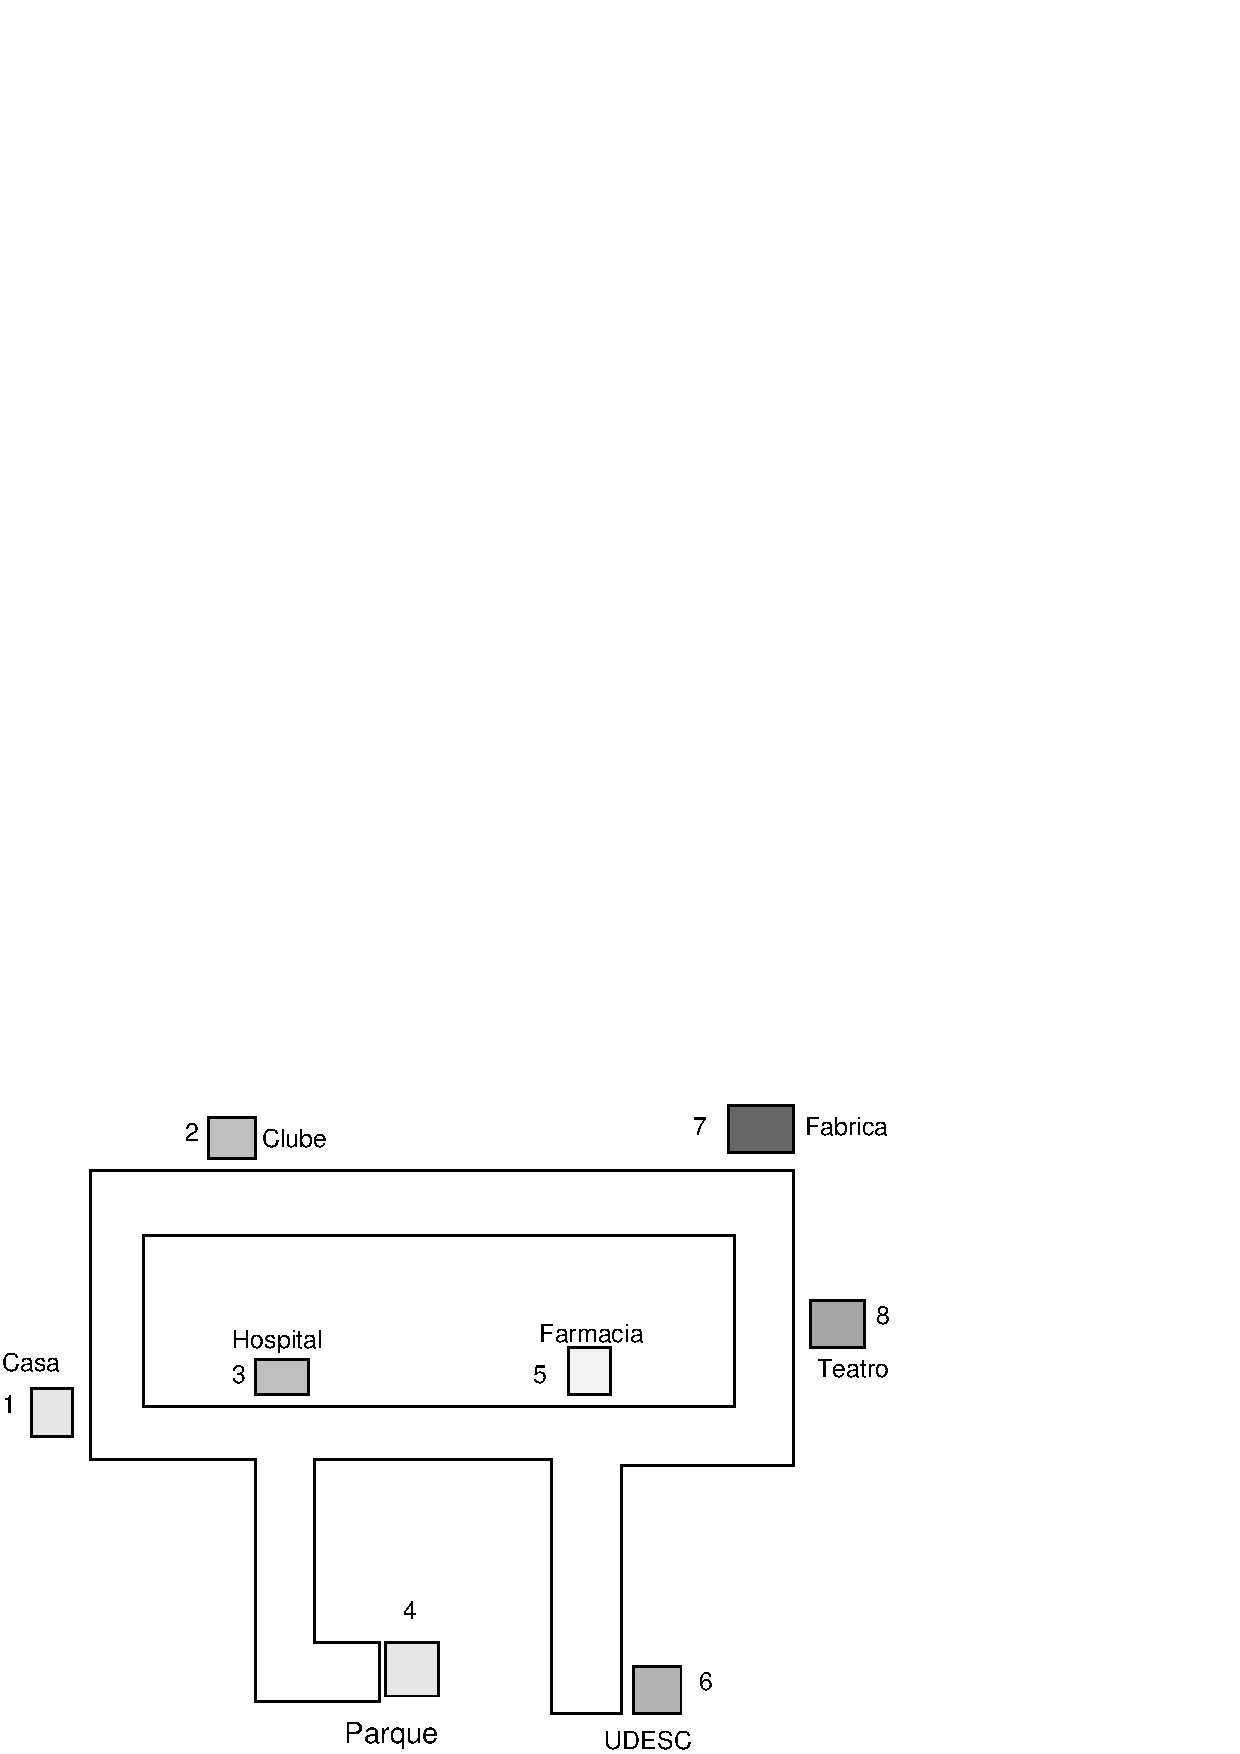
\includegraphics[scale=0.5]{figuras/grafo_mapa.pdf}
%%Prolog/
\label{fig_grafo_mapa}
\caption{Um mapa - grafo clássico}
\end{figure}


\end{frame}

%%%%%%%%%%%%%%%%%%%%%%%%%%%%%%%%%%%%%%%%%%%

\begin{frame}[fragile]   %%%% indica que o ambiente  FRAME é frágil
\frametitle{Link dos códigos}
\begin{block}{Github:}
\begin{itemize}

  \item \url{https://github.com/claudiosa/Prolog/blob/master/mapa_cidade_largura.pl}
  \item \url{https://github.com/claudiosa/Prolog/blob/master/mapa_cidade_profundidade.pl}

\end{itemize}  
\end{block}   
\end{frame}

%%%%%%%%%%%%%%%%%%%%%%%%%%%%%%%%%%%%%%%

\section{Predicados Extra-Lógicos}
\begin{frame}

\frametitle{Predicados Extra-Lógicos}
\begin{block}{Exemplos:}

\lstinputlisting[language=Prolog, 
                  basicstyle=\footnotesize\ttfamily,
                  backgroundcolor=\color{azulclaro}, 
                  keywordstyle=\color{red},   
                  keepspaces=true, 
                  lineskip = -2pt, % espacamento entre linhas
%%                  numbersep=5pt   
                  keywordstyle=\color{magenta},
     numberstyle=\tiny\color{magenta},
     commentstyle=\color{green},             
    numbers=left, 
    captionpos = b, % posiaodo caption 
    label={lista},                 
    ]{prolog/predicados.txt}

\end{block}
\end{frame}

%%%%%%%%%%%%%%%%%%%%%%%%%%%%%%%%%%%%%%%

\begin{frame}
\frametitle{Predicados \textit{Mão-na-Roda}}

\begin{block}{Exemplos:}

{\scriptsize
\inputminted{Prolog}{prolog/predicados2.txt}
}
    
\end{block}
\end{frame}

%%%%%%%%%%%%%%%%%%%%%%%%%%%%%%%%%%%%%%%

\begin{frame}
\frametitle{Predicados \textit{Mão-na-Roda}}

\begin{block}{Dica:}

 Os detalhes de uso deles voce descobre via {\tt ?- help} e {\tt apropos}, manual  e exemplos
via {\em Google}.



\end{block}
\end{frame}

%%%%%%%%%%%%%%%%%%%%%%%%%%%%%%%%%%%%%%%

\begin{comment}
\section{Outros Aspectos}
\frametitle{Outros Aspectos}
\begin{frame}
\begin{block}{If then etc}

Gerando executáveis\\
assert retract


\end{block}
\end{frame}
\end{comment}

%%%%%%%%%%%%%%%%%%%%%%%%%%%%%%%%%%%%%%%%%
\begin{frame}
\begin{block}{Dicas de Programação}
\begin{itemize}

\item Tenha um editor sensível a sintaxe do Prolog. Isto ajuda
muito aos iniciantes.

\item Ao carregar o programa no interpretador, certifique-se
que não existam erros. Senão o código com erro não é carregado completamente.

\item Evite ficar pensando obstinadamente sobre um predicado
que está dando problema. Faça uma abordagem nova ou {\em vá andando}.
Respire, saia de frente do computador, oxalá!

\item Cuidado ao dar nomes de variáveis. Use nomes significativos
e curtos.

\item Cuidar nos predicados proibidos de {\em backtraking}. Exemplo
é o {\tt is}. Veja o que fazer para contornar, por exemplo:

\end{itemize}

\lstinputlisting[language=Prolog, 
                  basicstyle=\footnotesize\ttfamily,
                  backgroundcolor=\color{azulclaro}, 
                  keywordstyle=\color{red},   
                  keepspaces=true, 
                  lineskip = -2pt, % espacamento entre linhas
%%                  numbersep=5pt   
                  keywordstyle=\color{magenta},
     numberstyle=\tiny\color{magenta},
     commentstyle=\color{green},             
    numbers=left, 
    captionpos = b, % posiaodo caption 
    label={lista},                 
    ]{prolog/lista7.txt}

\end{block}
\end{frame}





%%%%%%%%%%%%%%%%%%%%%%%%%%%%%%%%%%%%%%%%%%%%%%%%
\section{Referências}
\subsection{Sites Interessantes}
\begin{frame}
\begin{block}{Sites Interessantes}
\begin{itemize}

%\setlength{\itemsep}{-3pt}
\item  \url{http://www.cse.unsw.edu.au/~billw/Prologdict.html} (Dicionário de Prolog)
%\item  \url{http://www.sju.edu/~jhodgson/ugai/}
%\item  \url{http://www.cee.hw.ac.uk/~alison/ai3notes/}
%\item  \url{http://dobrev.com/download.html}
\item  \url{http://www.swi-prolog.org/}
%\item  http://swi.psy.uva.nl/projects/xpce/download.html
\item  \url{http://www.amzi.com} (tem vários artigos e tutoriais
  que ilustram o uso e aprendizado do Prolog, respectivamente. Um site fortemente recomendado, incluindo  um ambiente de programação.)
\item  \url{http://www.arity.com} tem um outro Prolog free
\item  \url{http://www.ida.liu.se/~ulfni/lpp/}
\item  Strawberry Prolog:  \url{http://www.dobrev.com/}

\end{itemize}
\end{block}
\end{frame}

%%%%%%%%%%%%%%%%%%%%%%%%%%%%%%%%%%%%%%%%%%%%%%%%

\subsection{Alguns Bons Livros}
\begin{frame}

\begin{block}{Alguns Bons Livros}

\begin{itemize}
%\setlength{\itemsep}{-3pt}
\item Michael A. Convigton, Donald
Nute, André Vellino; {\em Prolog - Programming in Depth},
Prentice-Hall, 1997;

\item Ivan Bratko; {\em Prolog, Programming
for Artificial Intelligence}, 2nd edition (or later if there is
one), Addison-Wesley;

\item W.F. Clocksin and C.S. Mellish;  {\em Programming in Prolog}, 3rd edition, Springer-Verlag;

\item Leon Sterling and Ehud Shapiro; {\em The Art of Prolog}, MIT Press;

\item Richard A. O'Keefe; {\em The Craft of Prolog}, MIT Press
1990;

\item  Há um título de um livro de IA, que é
``{\em aproximadamente}'' é: ``{\em Solving Complexs Problems with Artificial
Intelligence}'',  cuja linguagem utilizada nas soluções é o Prolog.


\end{itemize}
\end{block}
\end{frame}

\end{document}
